% Options for packages loaded elsewhere
\PassOptionsToPackage{unicode}{hyperref}
\PassOptionsToPackage{hyphens}{url}
\PassOptionsToPackage{dvipsnames,svgnames,x11names}{xcolor}
%
\documentclass[
  8pt,
  ignorenonframetext,
  aspectratio=169]{beamer}
\title{Crash course: Geospatial Datavisualisering}
\author{Jeppe Vierø}
\date{\today}

\usepackage{pgfpages}
\setbeamertemplate{caption}[numbered]
\setbeamertemplate{caption label separator}{: }
\setbeamercolor{caption name}{fg=normal text.fg}
\beamertemplatenavigationsymbolsempty
% Prevent slide breaks in the middle of a paragraph
\widowpenalties 1 10000
\raggedbottom
\setbeamertemplate{part page}{
  \centering
  \begin{beamercolorbox}[sep=16pt,center]{part title}
    \usebeamerfont{part title}\insertpart\par
  \end{beamercolorbox}
}
\setbeamertemplate{section page}{
  \centering
  \begin{beamercolorbox}[sep=12pt,center]{part title}
    \usebeamerfont{section title}\insertsection\par
  \end{beamercolorbox}
}
\setbeamertemplate{subsection page}{
  \centering
  \begin{beamercolorbox}[sep=8pt,center]{part title}
    \usebeamerfont{subsection title}\insertsubsection\par
  \end{beamercolorbox}
}
\AtBeginPart{
  \frame{\partpage}
}
\AtBeginSection{
  \ifbibliography
  \else
    \frame{\sectionpage}
  \fi
}
\AtBeginSubsection{
  \frame{\subsectionpage}
}
\usepackage{amsmath,amssymb}
\usepackage{lmodern}
\usepackage{iftex}
\ifPDFTeX
  \usepackage[T1]{fontenc}
  \usepackage[utf8]{inputenc}
  \usepackage{textcomp} % provide euro and other symbols
\else % if luatex or xetex
  \usepackage{unicode-math}
  \defaultfontfeatures{Scale=MatchLowercase}
  \defaultfontfeatures[\rmfamily]{Ligatures=TeX,Scale=1}
\fi
\usetheme[]{CambridgeUS}
% Use upquote if available, for straight quotes in verbatim environments
\IfFileExists{upquote.sty}{\usepackage{upquote}}{}
\IfFileExists{microtype.sty}{% use microtype if available
  \usepackage[]{microtype}
  \UseMicrotypeSet[protrusion]{basicmath} % disable protrusion for tt fonts
}{}
\makeatletter
\@ifundefined{KOMAClassName}{% if non-KOMA class
  \IfFileExists{parskip.sty}{%
    \usepackage{parskip}
  }{% else
    \setlength{\parindent}{0pt}
    \setlength{\parskip}{6pt plus 2pt minus 1pt}}
}{% if KOMA class
  \KOMAoptions{parskip=half}}
\makeatother
\usepackage{xcolor}
\IfFileExists{xurl.sty}{\usepackage{xurl}}{} % add URL line breaks if available
\IfFileExists{bookmark.sty}{\usepackage{bookmark}}{\usepackage{hyperref}}
\hypersetup{
  pdftitle={Crash course: Geospatial Datavisualisering},
  pdfauthor={Jeppe Vierø},
  colorlinks=true,
  linkcolor={Maroon},
  filecolor={Maroon},
  citecolor={Blue},
  urlcolor={blue},
  pdfcreator={LaTeX via pandoc}}
\urlstyle{same} % disable monospaced font for URLs
\newif\ifbibliography
\usepackage{color}
\usepackage{fancyvrb}
\newcommand{\VerbBar}{|}
\newcommand{\VERB}{\Verb[commandchars=\\\{\}]}
\DefineVerbatimEnvironment{Highlighting}{Verbatim}{commandchars=\\\{\}}
% Add ',fontsize=\small' for more characters per line
\newenvironment{Shaded}{}{}
\newcommand{\AlertTok}[1]{\textcolor[rgb]{1.00,0.00,0.00}{\textbf{#1}}}
\newcommand{\AnnotationTok}[1]{\textcolor[rgb]{0.38,0.63,0.69}{\textbf{\textit{#1}}}}
\newcommand{\AttributeTok}[1]{\textcolor[rgb]{0.49,0.56,0.16}{#1}}
\newcommand{\BaseNTok}[1]{\textcolor[rgb]{0.25,0.63,0.44}{#1}}
\newcommand{\BuiltInTok}[1]{#1}
\newcommand{\CharTok}[1]{\textcolor[rgb]{0.25,0.44,0.63}{#1}}
\newcommand{\CommentTok}[1]{\textcolor[rgb]{0.38,0.63,0.69}{\textit{#1}}}
\newcommand{\CommentVarTok}[1]{\textcolor[rgb]{0.38,0.63,0.69}{\textbf{\textit{#1}}}}
\newcommand{\ConstantTok}[1]{\textcolor[rgb]{0.53,0.00,0.00}{#1}}
\newcommand{\ControlFlowTok}[1]{\textcolor[rgb]{0.00,0.44,0.13}{\textbf{#1}}}
\newcommand{\DataTypeTok}[1]{\textcolor[rgb]{0.56,0.13,0.00}{#1}}
\newcommand{\DecValTok}[1]{\textcolor[rgb]{0.25,0.63,0.44}{#1}}
\newcommand{\DocumentationTok}[1]{\textcolor[rgb]{0.73,0.13,0.13}{\textit{#1}}}
\newcommand{\ErrorTok}[1]{\textcolor[rgb]{1.00,0.00,0.00}{\textbf{#1}}}
\newcommand{\ExtensionTok}[1]{#1}
\newcommand{\FloatTok}[1]{\textcolor[rgb]{0.25,0.63,0.44}{#1}}
\newcommand{\FunctionTok}[1]{\textcolor[rgb]{0.02,0.16,0.49}{#1}}
\newcommand{\ImportTok}[1]{#1}
\newcommand{\InformationTok}[1]{\textcolor[rgb]{0.38,0.63,0.69}{\textbf{\textit{#1}}}}
\newcommand{\KeywordTok}[1]{\textcolor[rgb]{0.00,0.44,0.13}{\textbf{#1}}}
\newcommand{\NormalTok}[1]{#1}
\newcommand{\OperatorTok}[1]{\textcolor[rgb]{0.40,0.40,0.40}{#1}}
\newcommand{\OtherTok}[1]{\textcolor[rgb]{0.00,0.44,0.13}{#1}}
\newcommand{\PreprocessorTok}[1]{\textcolor[rgb]{0.74,0.48,0.00}{#1}}
\newcommand{\RegionMarkerTok}[1]{#1}
\newcommand{\SpecialCharTok}[1]{\textcolor[rgb]{0.25,0.44,0.63}{#1}}
\newcommand{\SpecialStringTok}[1]{\textcolor[rgb]{0.73,0.40,0.53}{#1}}
\newcommand{\StringTok}[1]{\textcolor[rgb]{0.25,0.44,0.63}{#1}}
\newcommand{\VariableTok}[1]{\textcolor[rgb]{0.10,0.09,0.49}{#1}}
\newcommand{\VerbatimStringTok}[1]{\textcolor[rgb]{0.25,0.44,0.63}{#1}}
\newcommand{\WarningTok}[1]{\textcolor[rgb]{0.38,0.63,0.69}{\textbf{\textit{#1}}}}
\usepackage{graphicx}
\makeatletter
\def\maxwidth{\ifdim\Gin@nat@width>\linewidth\linewidth\else\Gin@nat@width\fi}
\def\maxheight{\ifdim\Gin@nat@height>\textheight\textheight\else\Gin@nat@height\fi}
\makeatother
% Scale images if necessary, so that they will not overflow the page
% margins by default, and it is still possible to overwrite the defaults
% using explicit options in \includegraphics[width, height, ...]{}
\setkeys{Gin}{width=\maxwidth,height=\maxheight,keepaspectratio}
% Set default figure placement to htbp
\makeatletter
\def\fps@figure{htbp}
\makeatother
\setlength{\emergencystretch}{3em} % prevent overfull lines
\providecommand{\tightlist}{%
  \setlength{\itemsep}{0pt}\setlength{\parskip}{0pt}}
\setcounter{secnumdepth}{-\maxdimen} % remove section numbering
\newcommand{\columnsbegin}{\begin{columns}}
\newcommand{\columnsend}{\end{columns}}


\AtBeginSection{
   \frame{\sectionpage}
}

\makeatletter
\setbeamertemplate{section page}
{
  \begingroup
    \centering
%    {\usebeamerfont{section name}\usebeamercolor[fg]{section name}\sectionname~\insertsectionnumber}
    \vskip1em\par
    \begin{beamercolorbox}[sep=12pt,center,colsep=-4bp,rounded=true,shadow=\beamer@themerounded@shadow]{section title}
      \usebeamerfont{section title}\insertsection\par
    \end{beamercolorbox}
  \endgroup
}
\makeatother


\usepackage{hyperref}
\ifLuaTeX
  \usepackage{selnolig}  % disable illegal ligatures
\fi

\begin{document}
\frame{\titlepage}

\begin{frame}[allowframebreaks]
  \tableofcontents[hideallsubsections]
\end{frame}
\begin{frame}
\tiny

\normalsize
\end{frame}

\hypertarget{introduktion}{%
\section{Introduktion}\label{introduktion}}

\begin{frame}{Motivation}
\protect\hypertarget{motivation}{}
\begin{figure}[H]
    \centering
    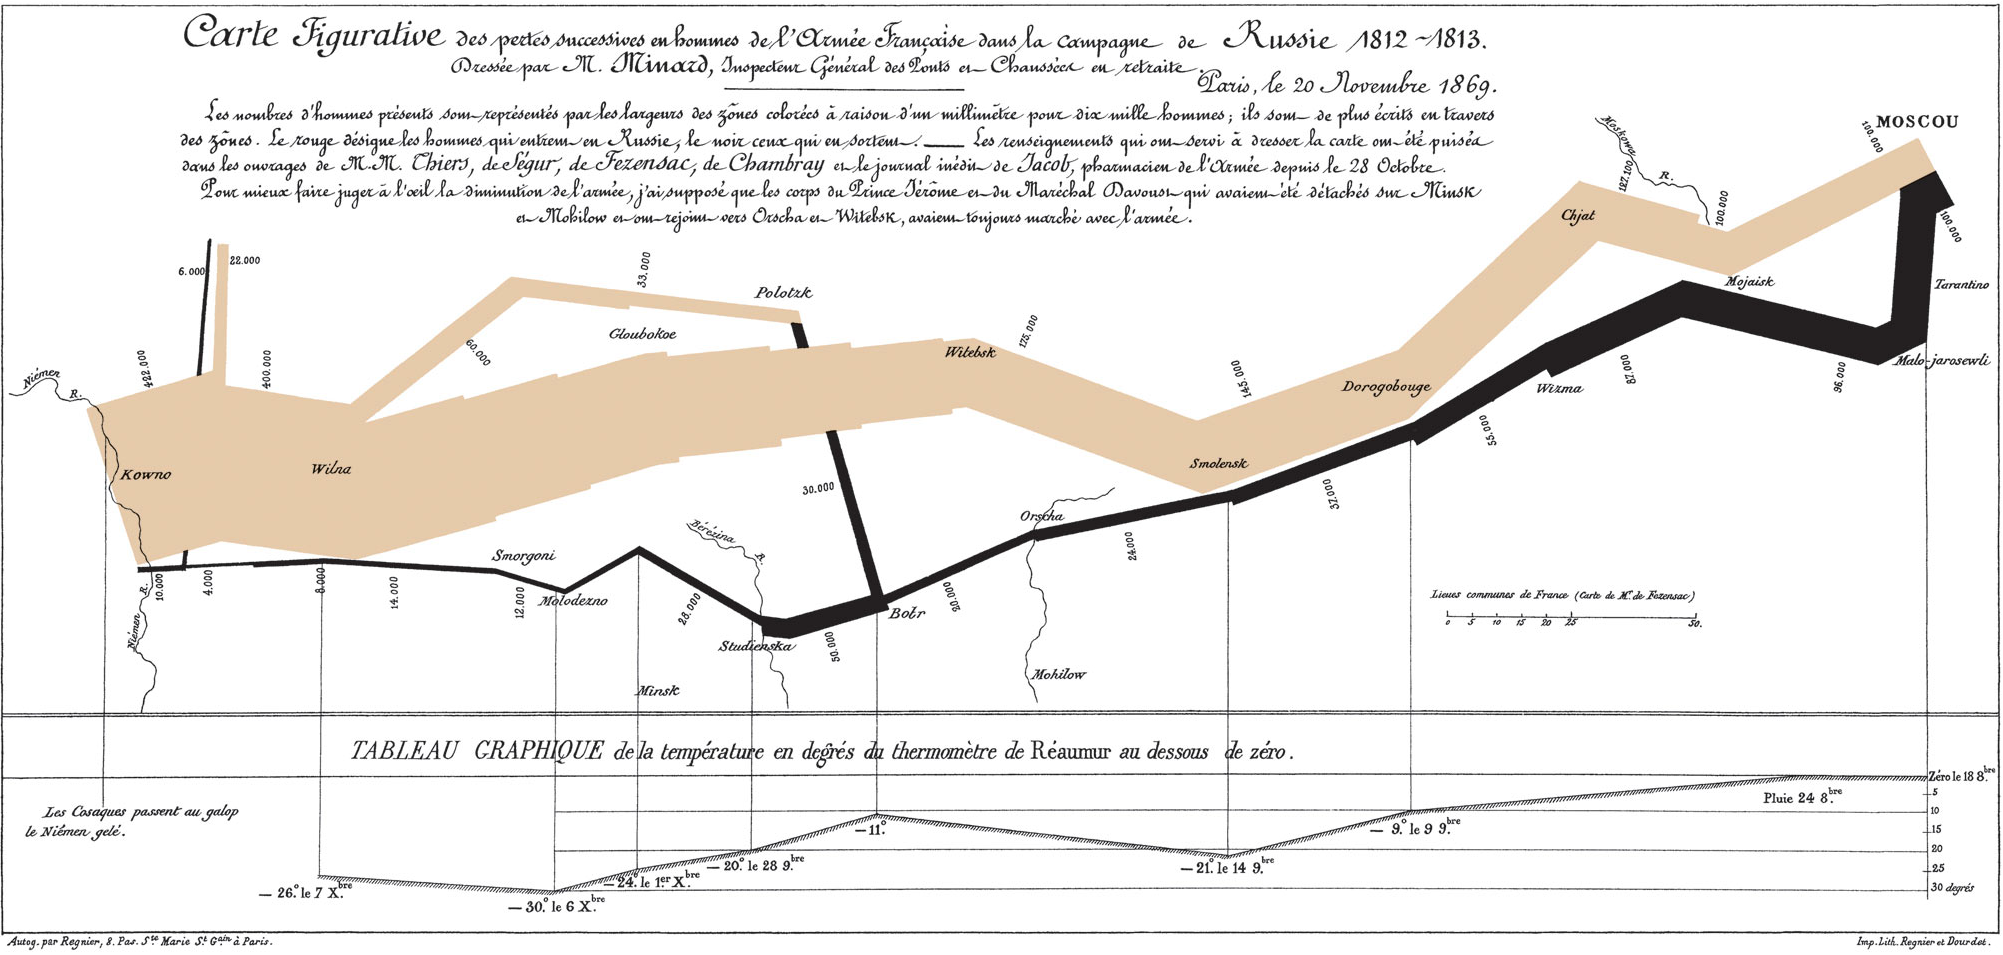
\includegraphics[width=.90\textwidth]{pictures/Minard.png}
    \caption{by Charles Joseph Minard, 1869}
\end{figure}
\end{frame}

\begin{frame}[fragile]{Afgrænsning}
\protect\hypertarget{afgruxe6nsning}{}
Jeg (regner med) at snakke \textbf{en del} om:

\begin{itemize}
\item
  Hvad \textbf{spatial} data er
\item
  Hvordan vi kan bruge spatiale datakilder til at \textbf{visualisere}
  andet data
\item
  Hvordan vi gør det i \texttt{R}
\end{itemize}

\bigskip

Jeg kommer \textbf{ikke} til at snakke (så meget) om:

\begin{itemize}
\item
  Datawrangling og -manipulation med geospatial data
\item
  Datavisualisering generelt
\end{itemize}
\end{frame}

\begin{frame}{Hvordan kan vi bruge geodata til at visualisere vores
pointer?}
\protect\hypertarget{hvordan-kan-vi-bruge-geodata-til-at-visualisere-vores-pointer}{}
\columnsbegin

\column{.5\textwidth}

\onslide <2->
\begin{figure}[H]
    \centering
    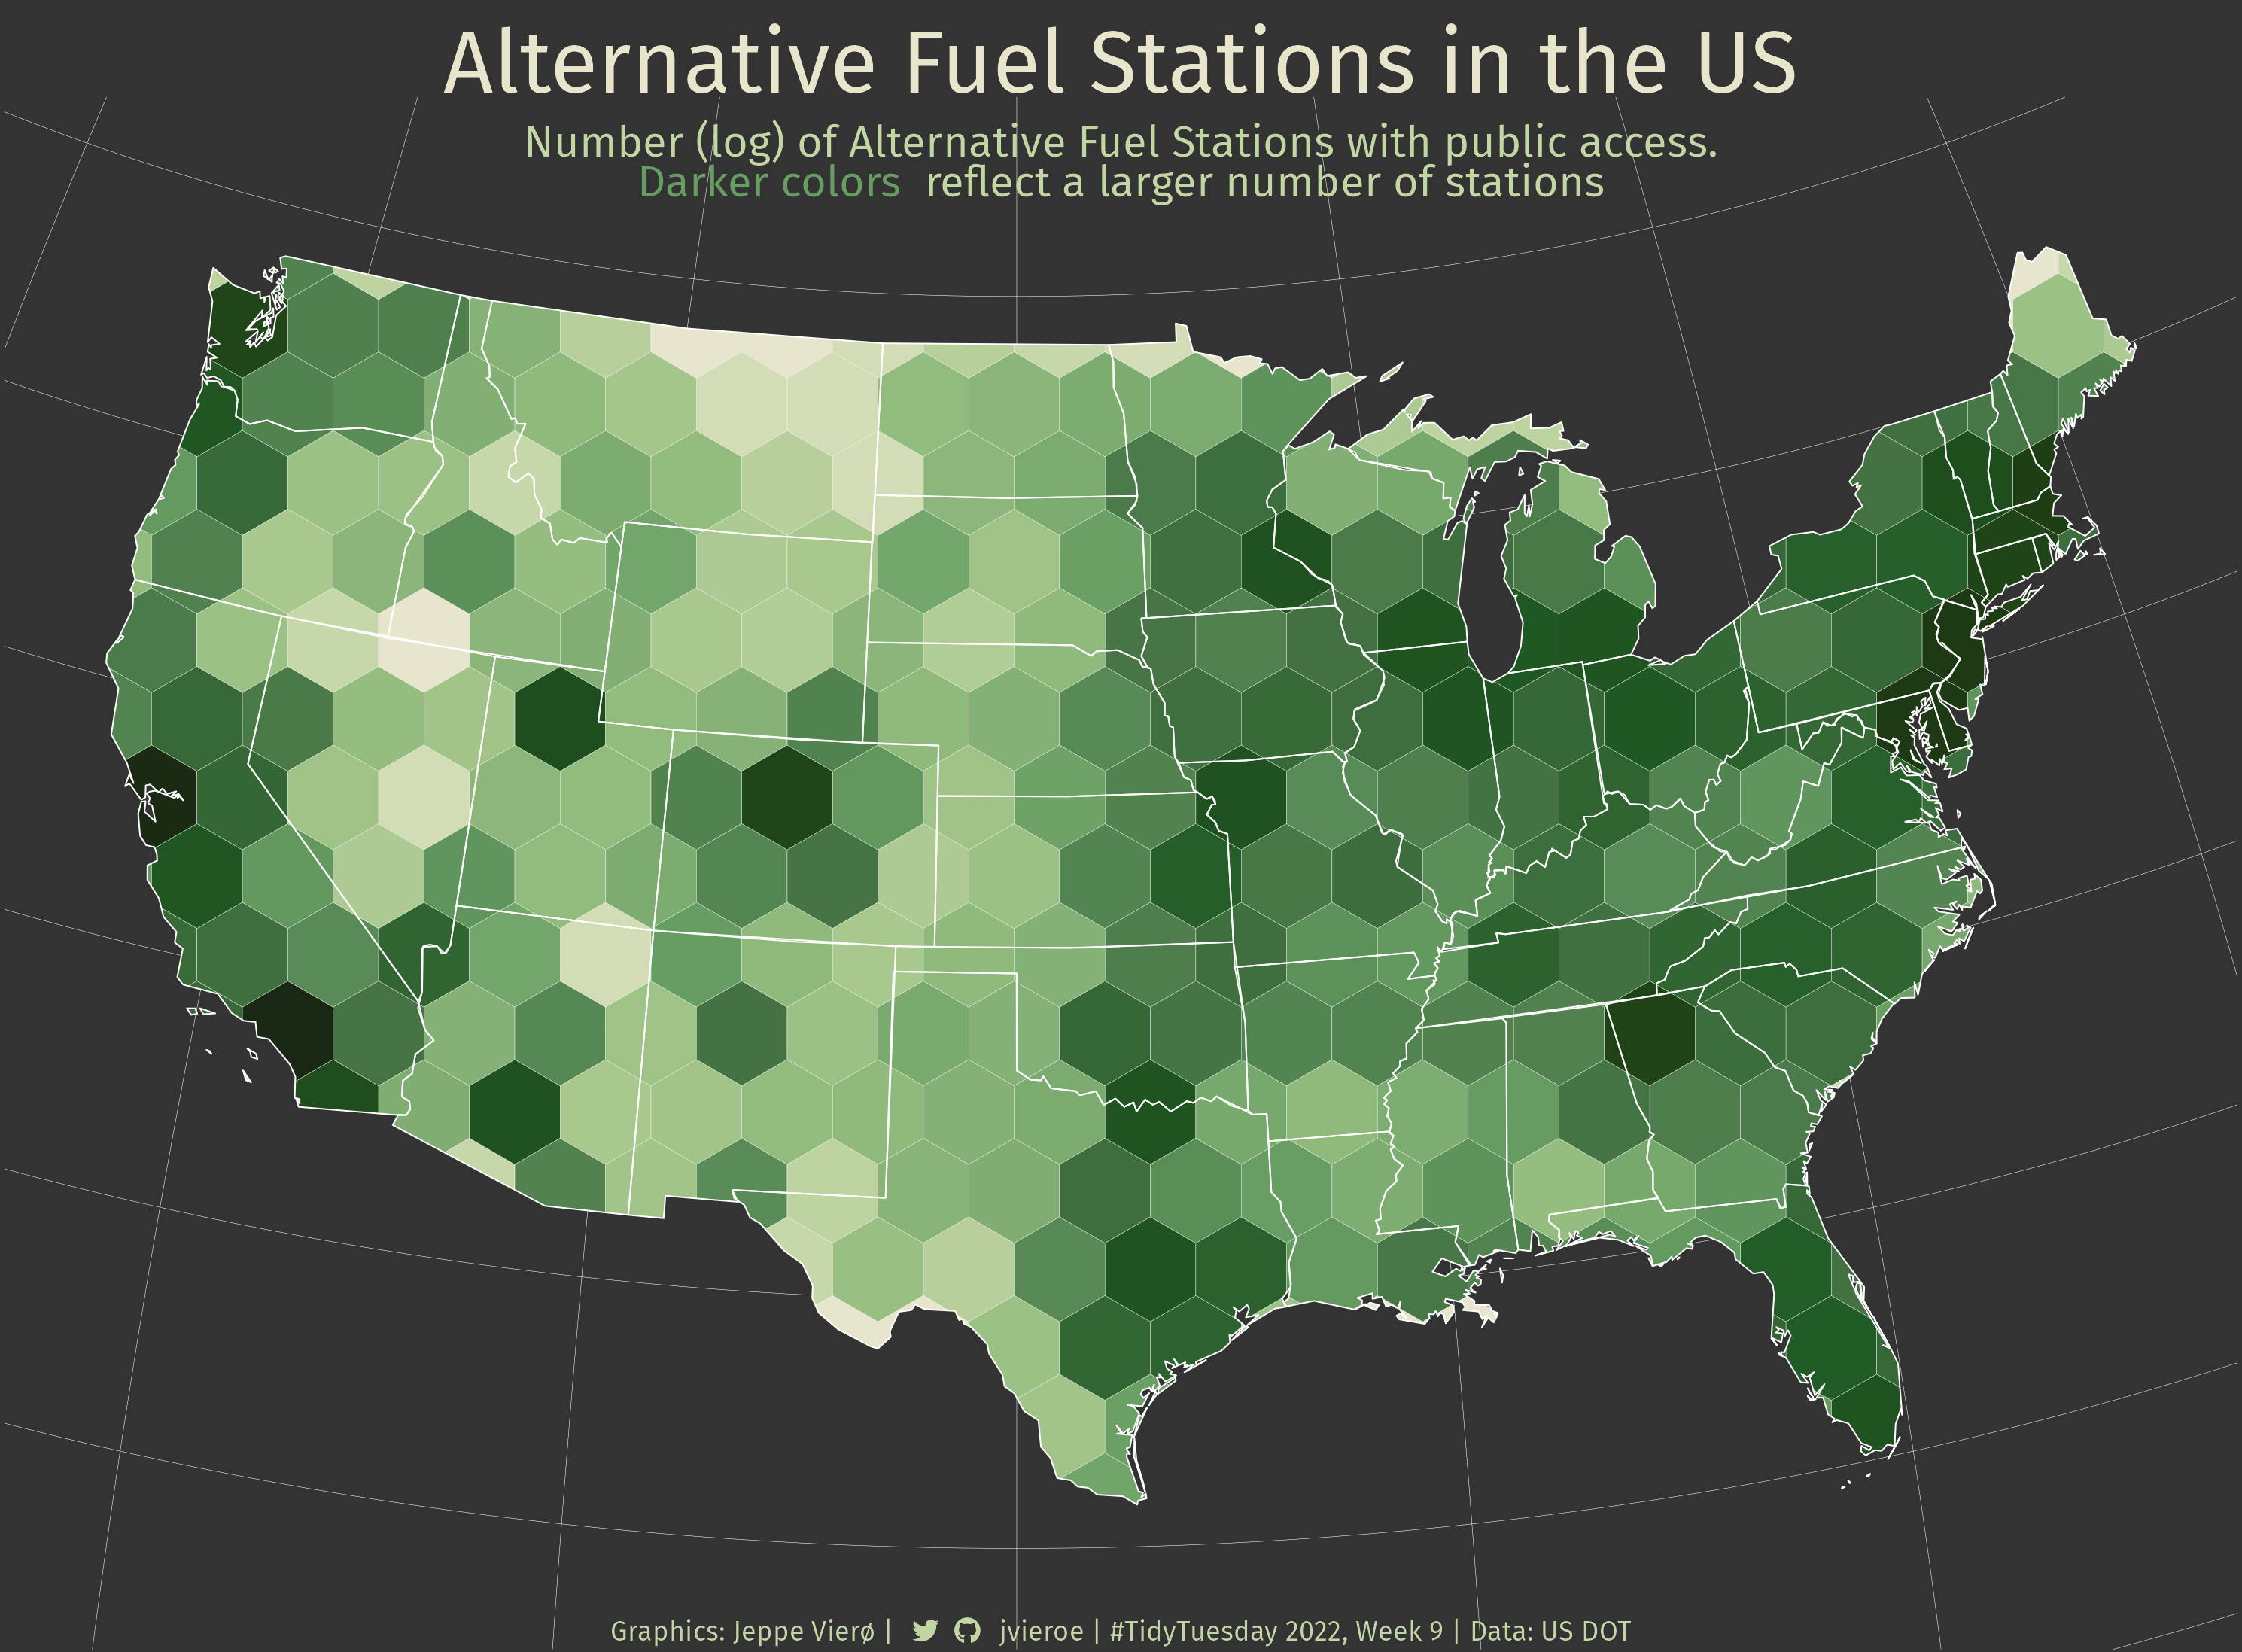
\includegraphics[width=.90\textwidth]{pictures/fuel.png}
\end{figure}

\column{.5\textwidth}

\onslide <3->
\begin{figure}[H]
    \centering
    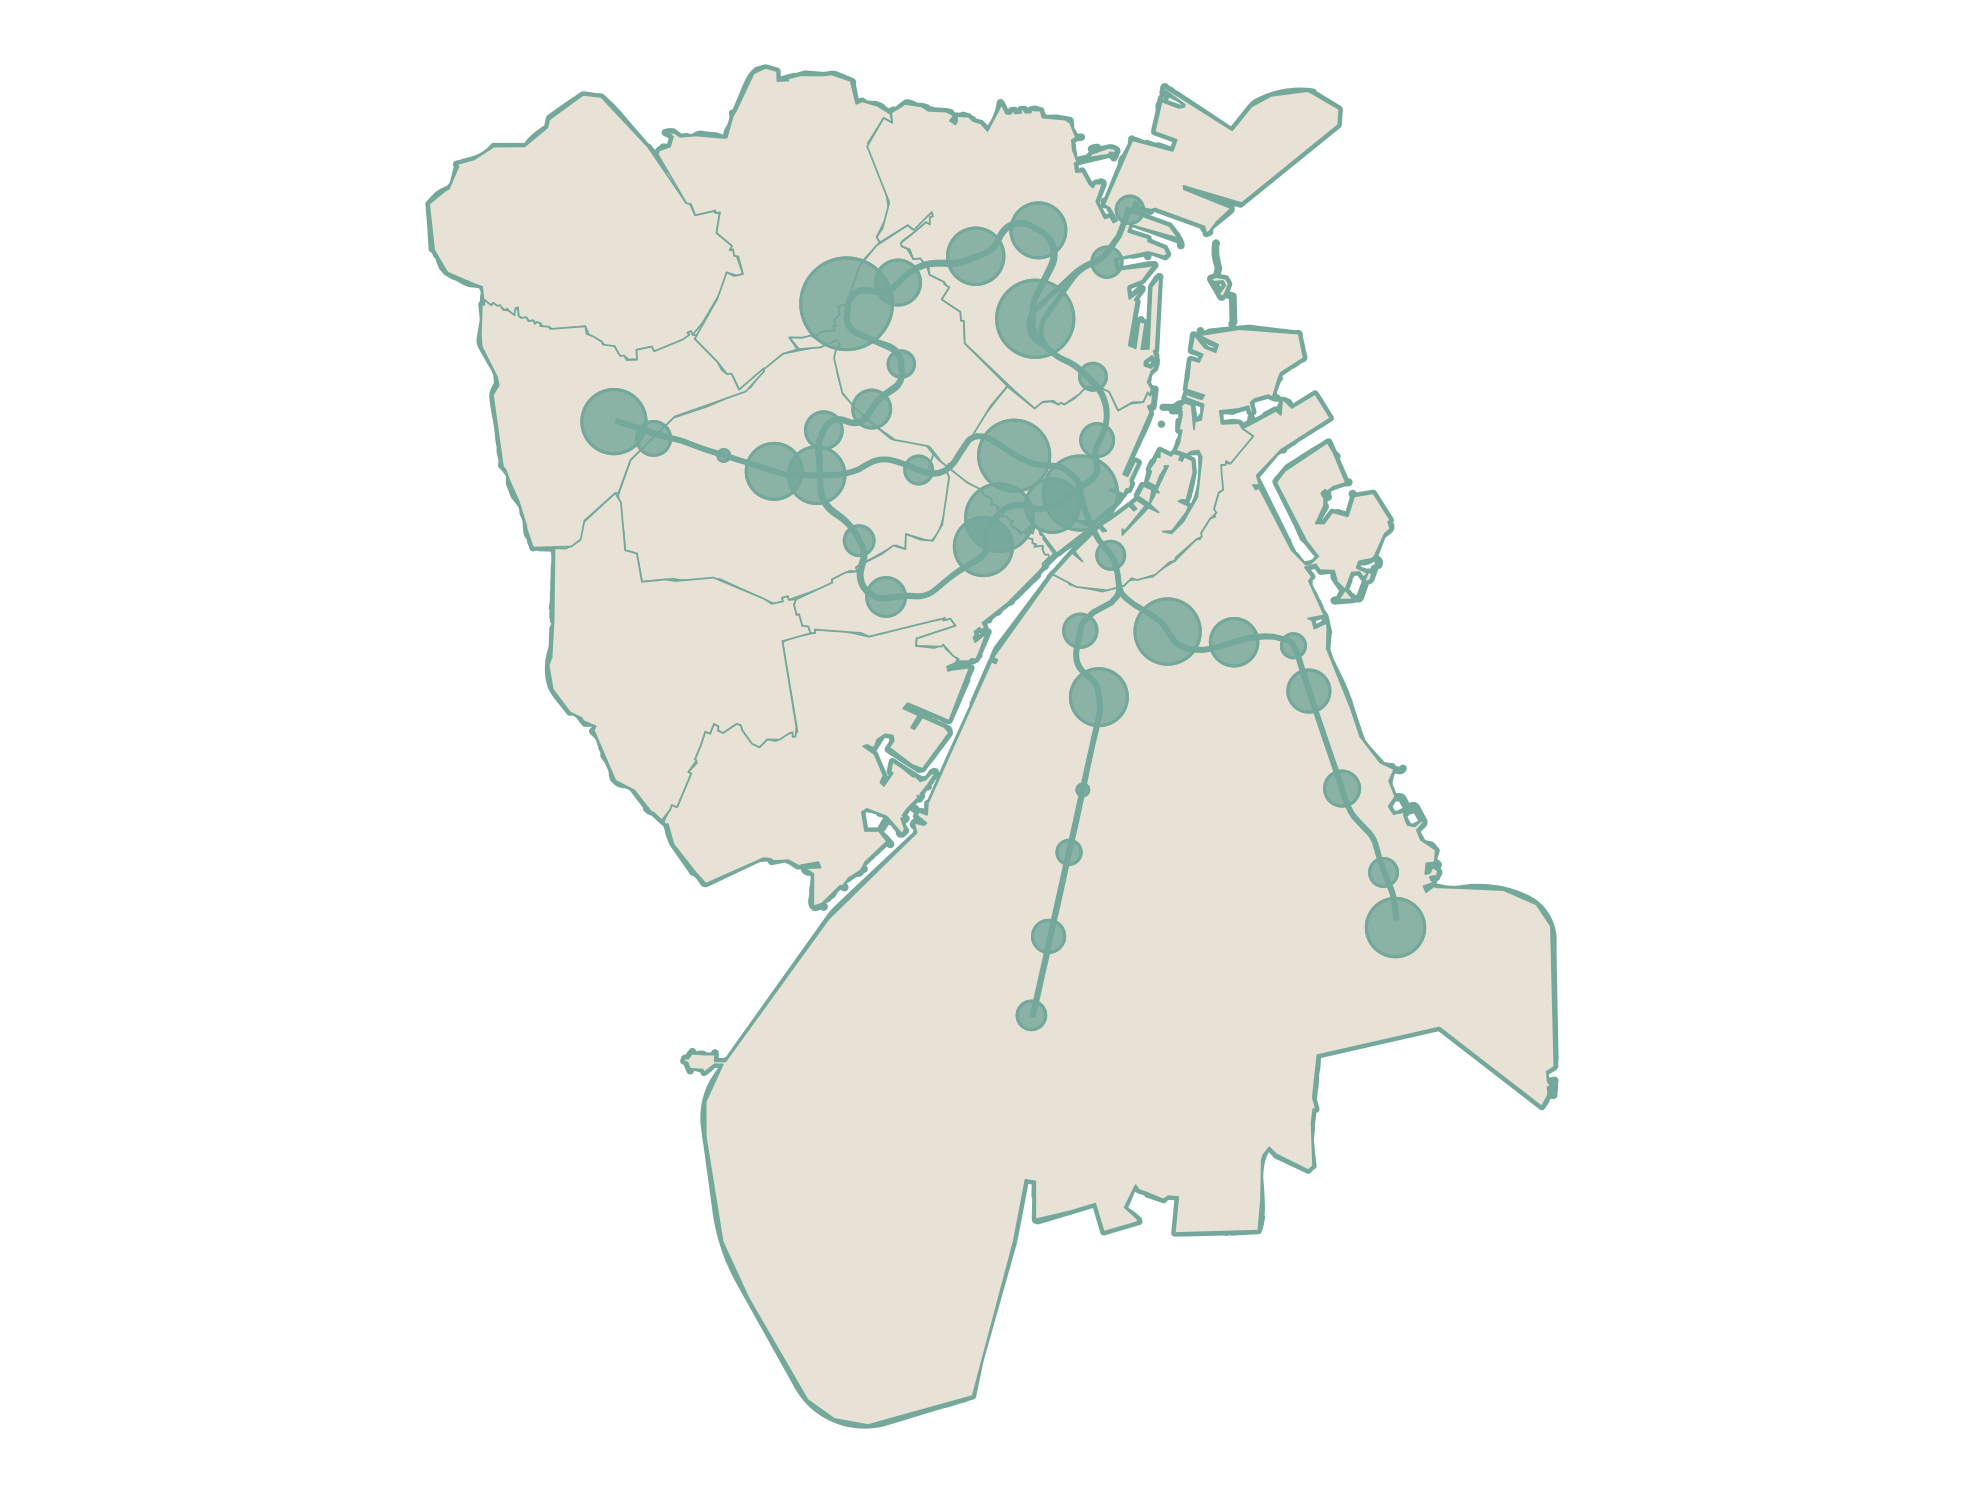
\includegraphics[width=.90\textwidth]{pictures/Forstadsbilister_start.png}
\end{figure}

\columnsend
\end{frame}

\begin{frame}{Hvordan kan vi bruge geodata til at visualisere vores
pointer?}
\protect\hypertarget{hvordan-kan-vi-bruge-geodata-til-at-visualisere-vores-pointer-1}{}
\columnsbegin

\column{.4\textwidth}

\onslide <1->
\begin{figure}[H]
    \centering
    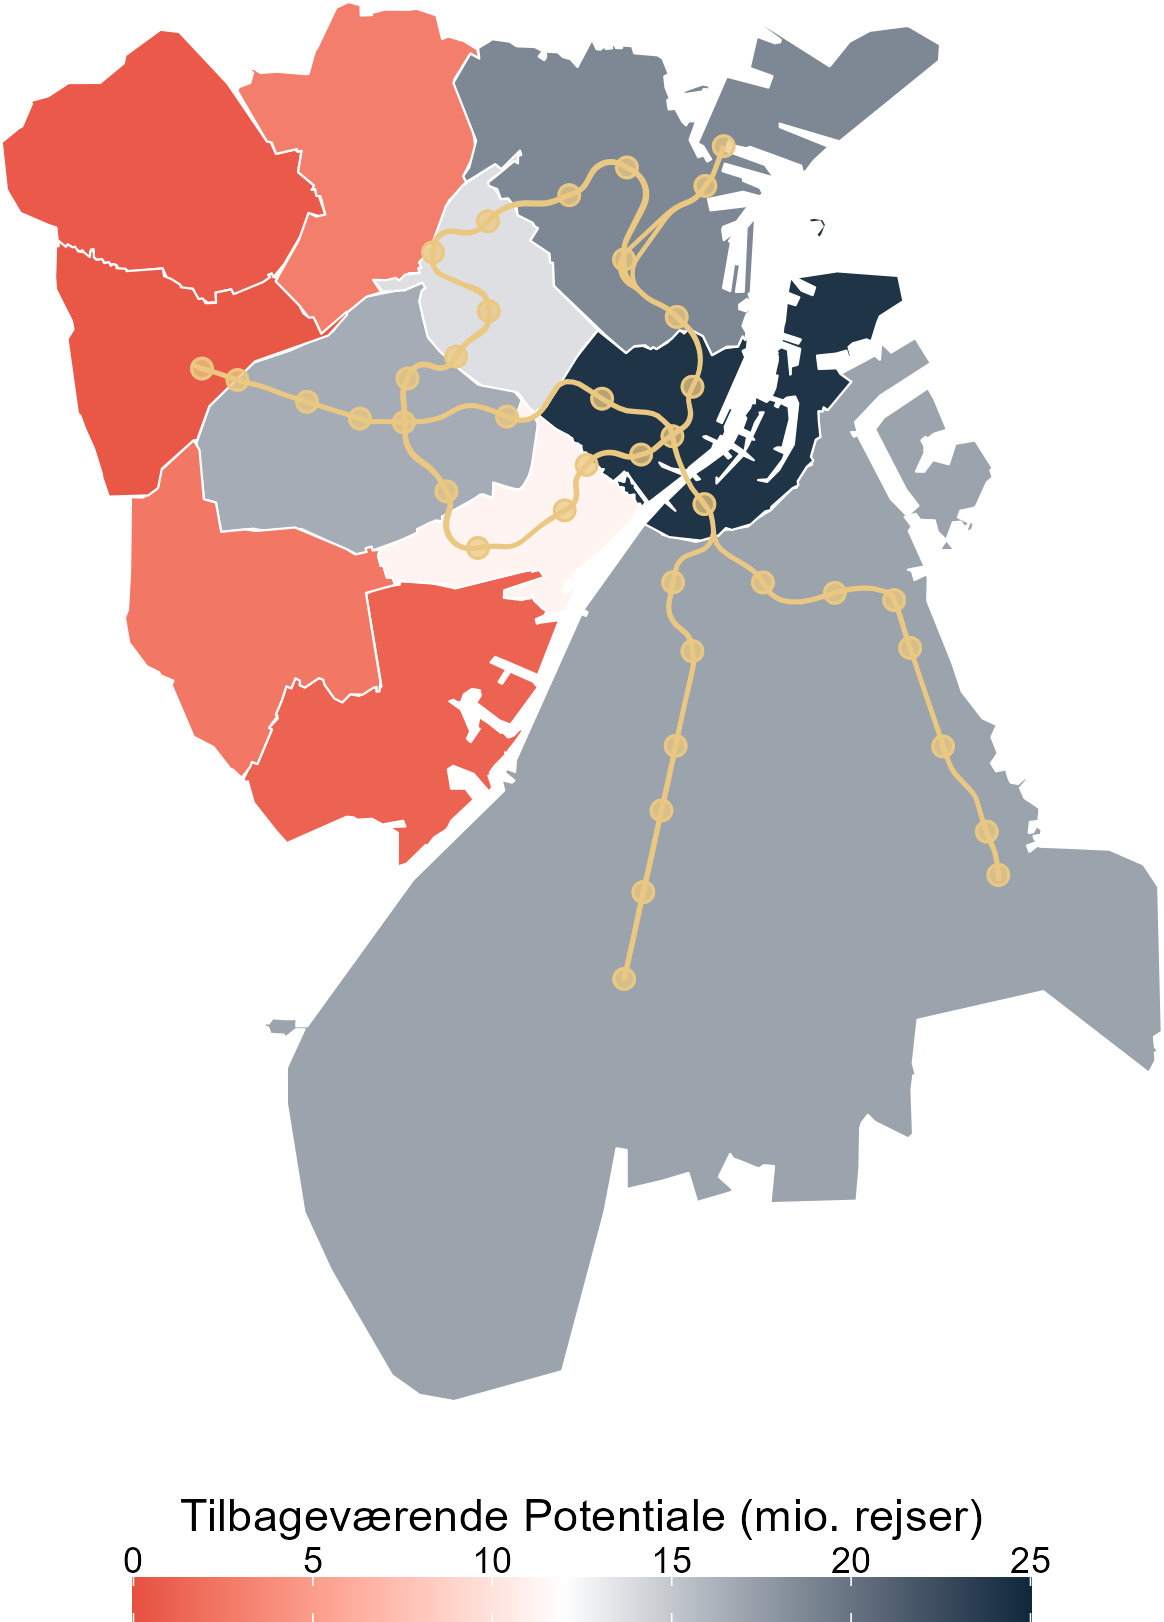
\includegraphics[width=.70\textwidth]{pictures/potentialeudnyttelse_absolut.png}
\end{figure}

\column{.6\textwidth}

\onslide <2->
\begin{figure}[H]
    \centering
    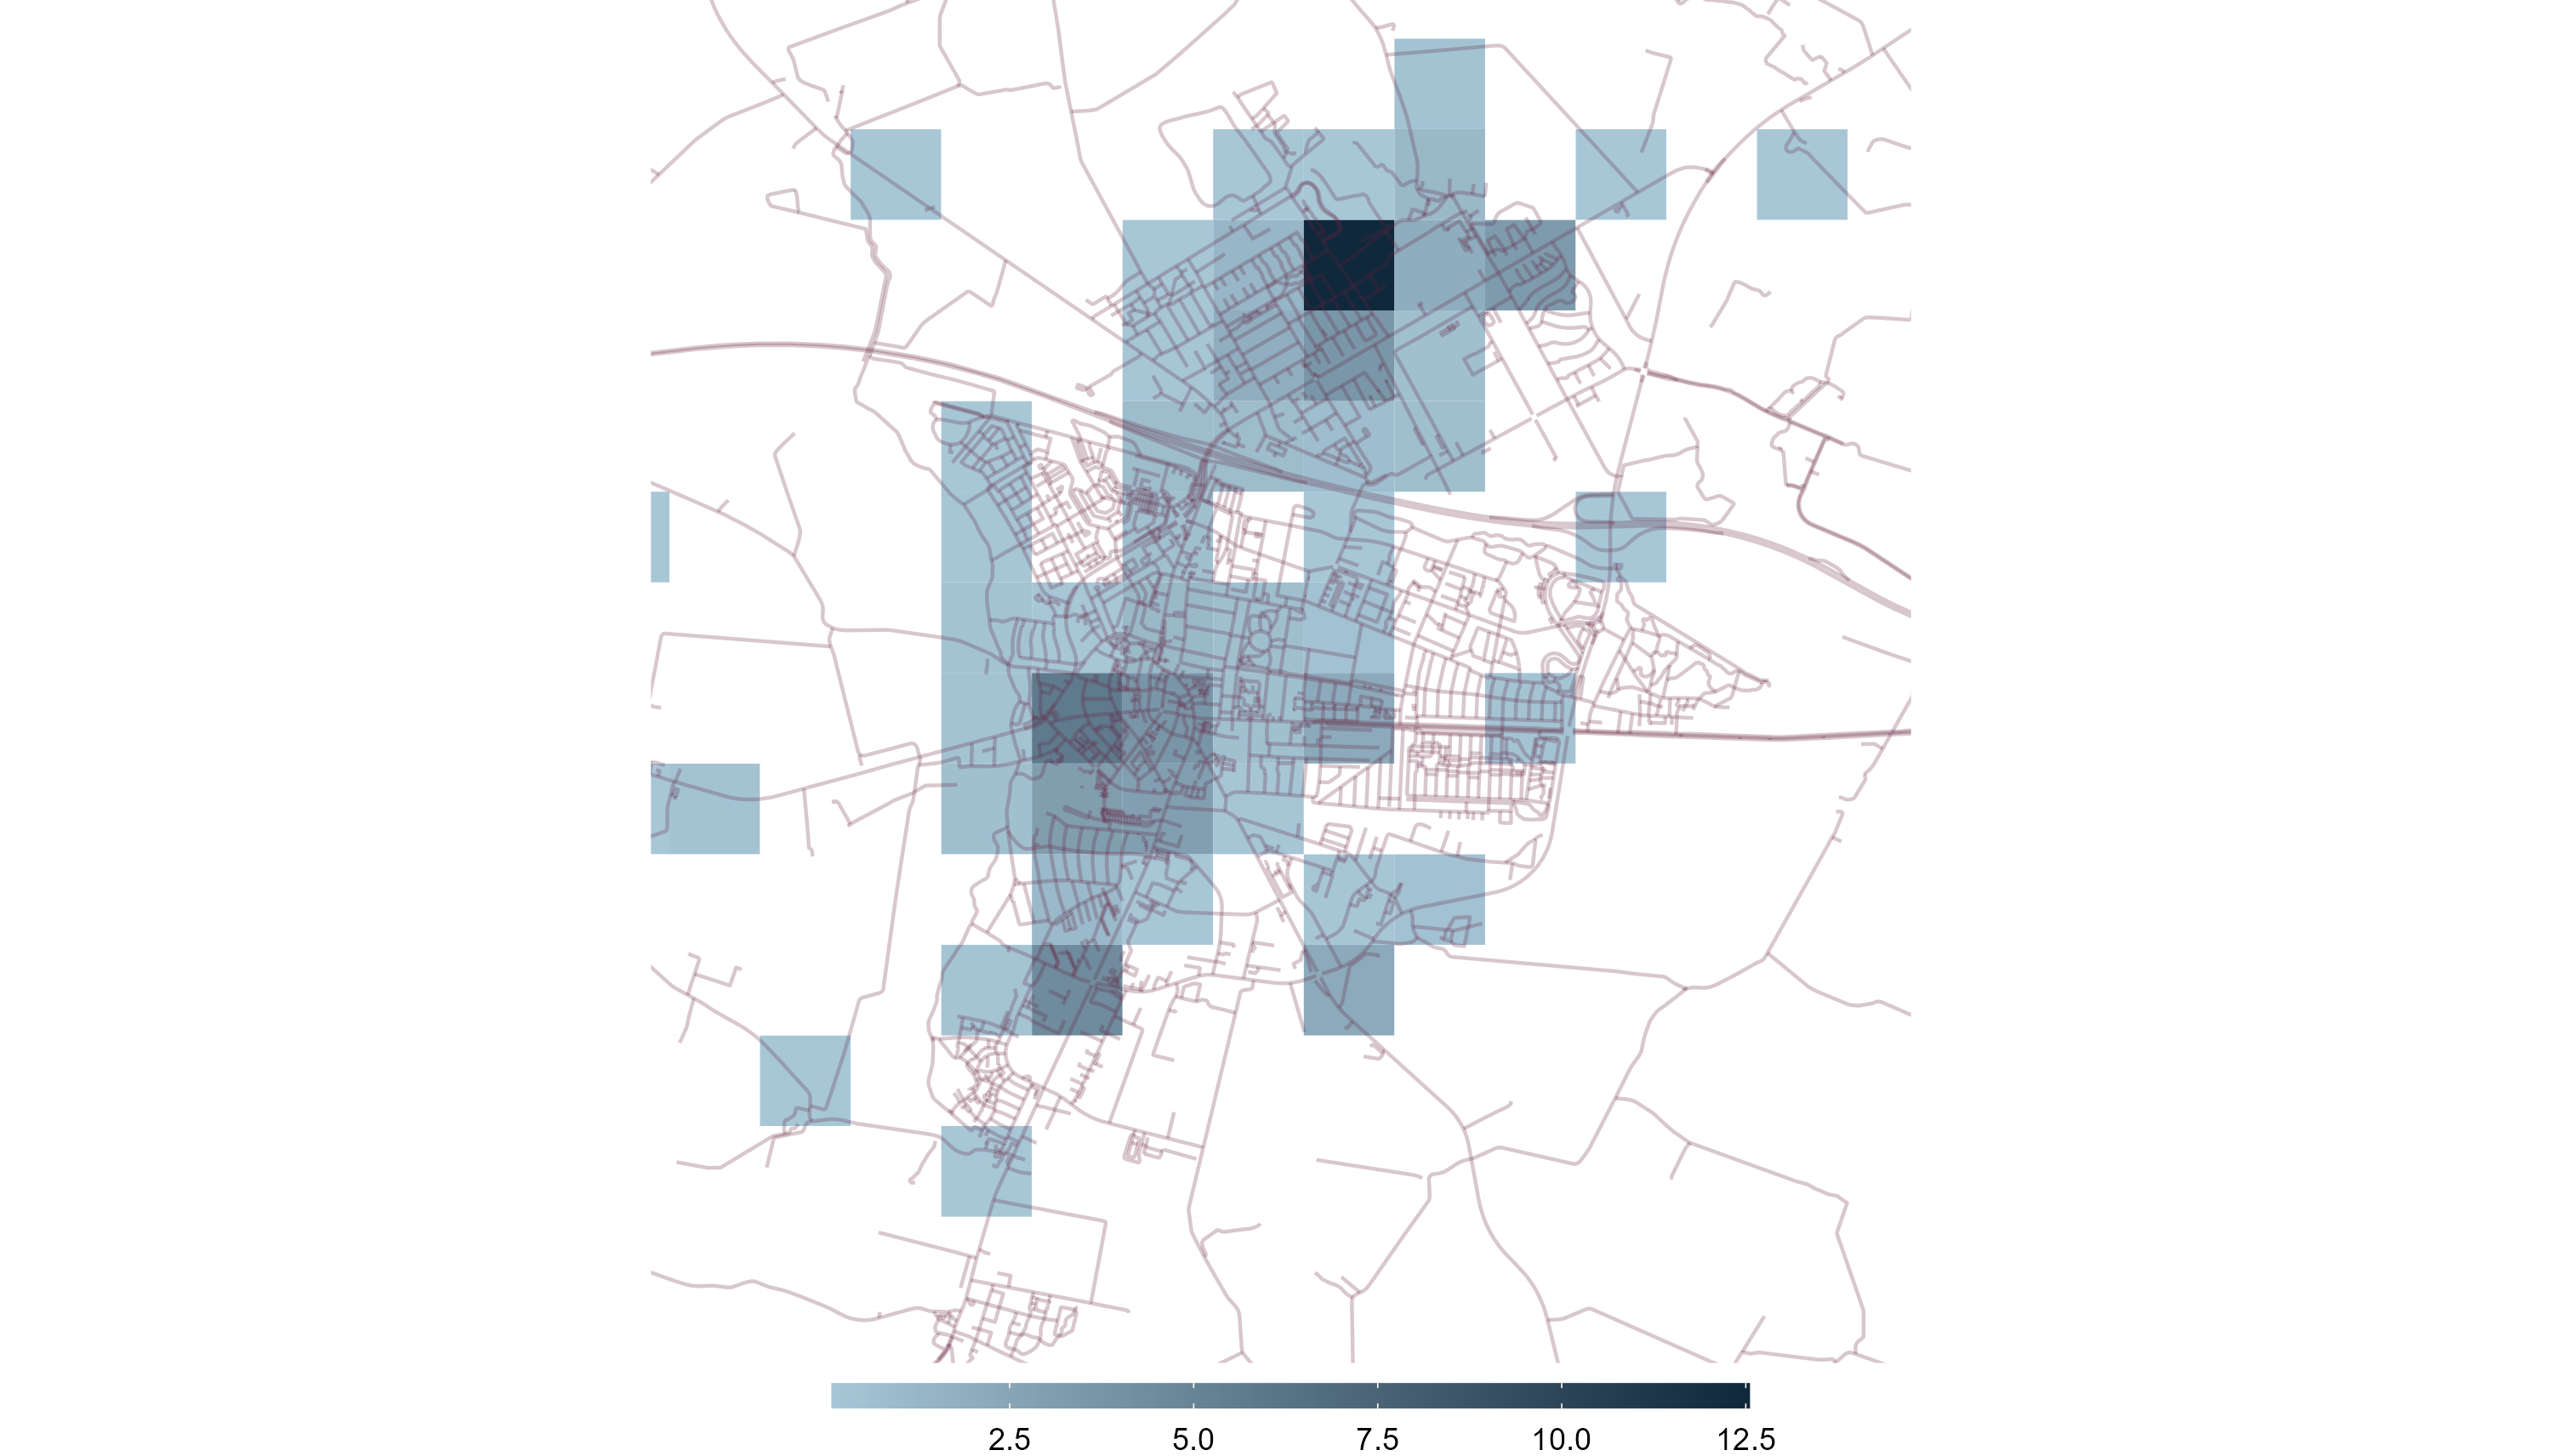
\includegraphics[width=.99\textwidth]{pictures/hex_ringsted.png}
\end{figure}

\columnsend
\end{frame}

\begin{frame}{Hvorfor ikke bare bruge ``klassiske'' visualiseringer?
(I)}
\protect\hypertarget{hvorfor-ikke-bare-bruge-klassiske-visualiseringer-i}{}
\columnsbegin
\column{.5\textwidth}

\tiny

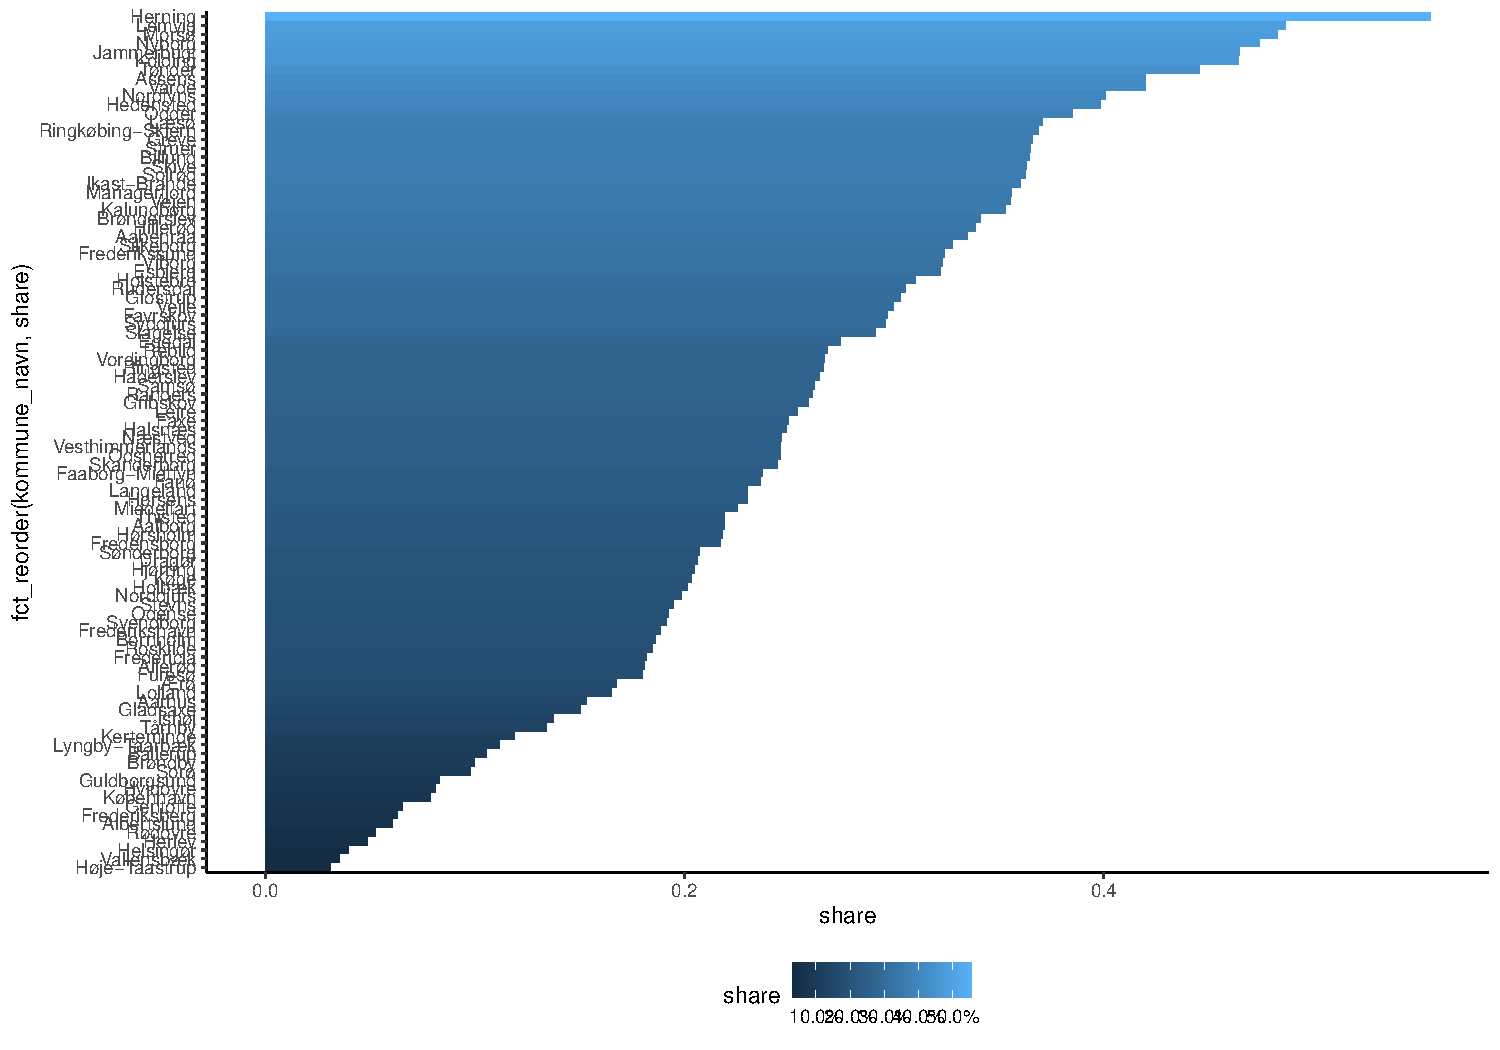
\includegraphics[width=1\linewidth]{crashcourse_slides_files/figure-beamer/unnamed-chunk-2-1}

\normalsize

\column{.5\textwidth}

\tiny

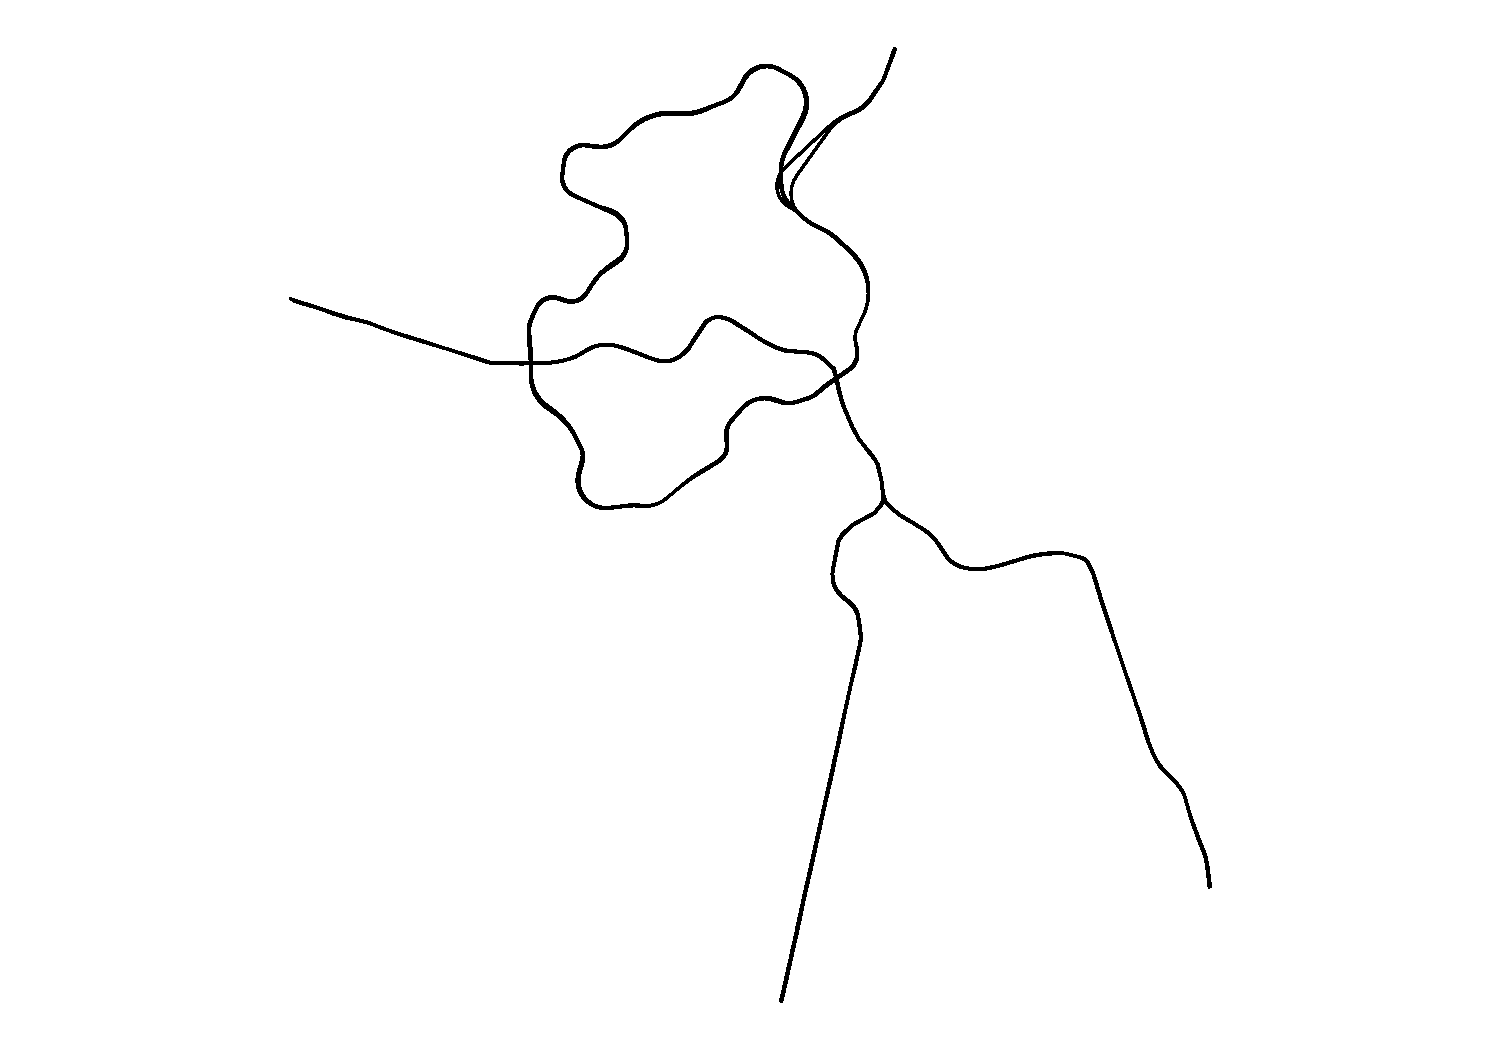
\includegraphics[width=1\linewidth]{crashcourse_slides_files/figure-beamer/unnamed-chunk-3-1}

\normalsize

\columnsend
\end{frame}

\begin{frame}{Hvorfor ikke bare bruge ``klassiske'' visualiseringer?
(II)}
\protect\hypertarget{hvorfor-ikke-bare-bruge-klassiske-visualiseringer-ii}{}
\columnsbegin

\column{.5\textwidth}

Typisk kan man med fordel (overveje at) visualisere sit data grafisk,
hvis

\begin{itemize}
\tightlist
\item
  Der er nogle \textbf{substantielle geografiske mønstre} i data, der er
  interessante (case in point:)
\end{itemize}

eller,

\begin{itemize}
\tightlist
\item
  Det data, vi gerne vil visualisere fundamentalt set har en geografisk
  dimension
\end{itemize}

\column{.5\textwidth}

\tiny

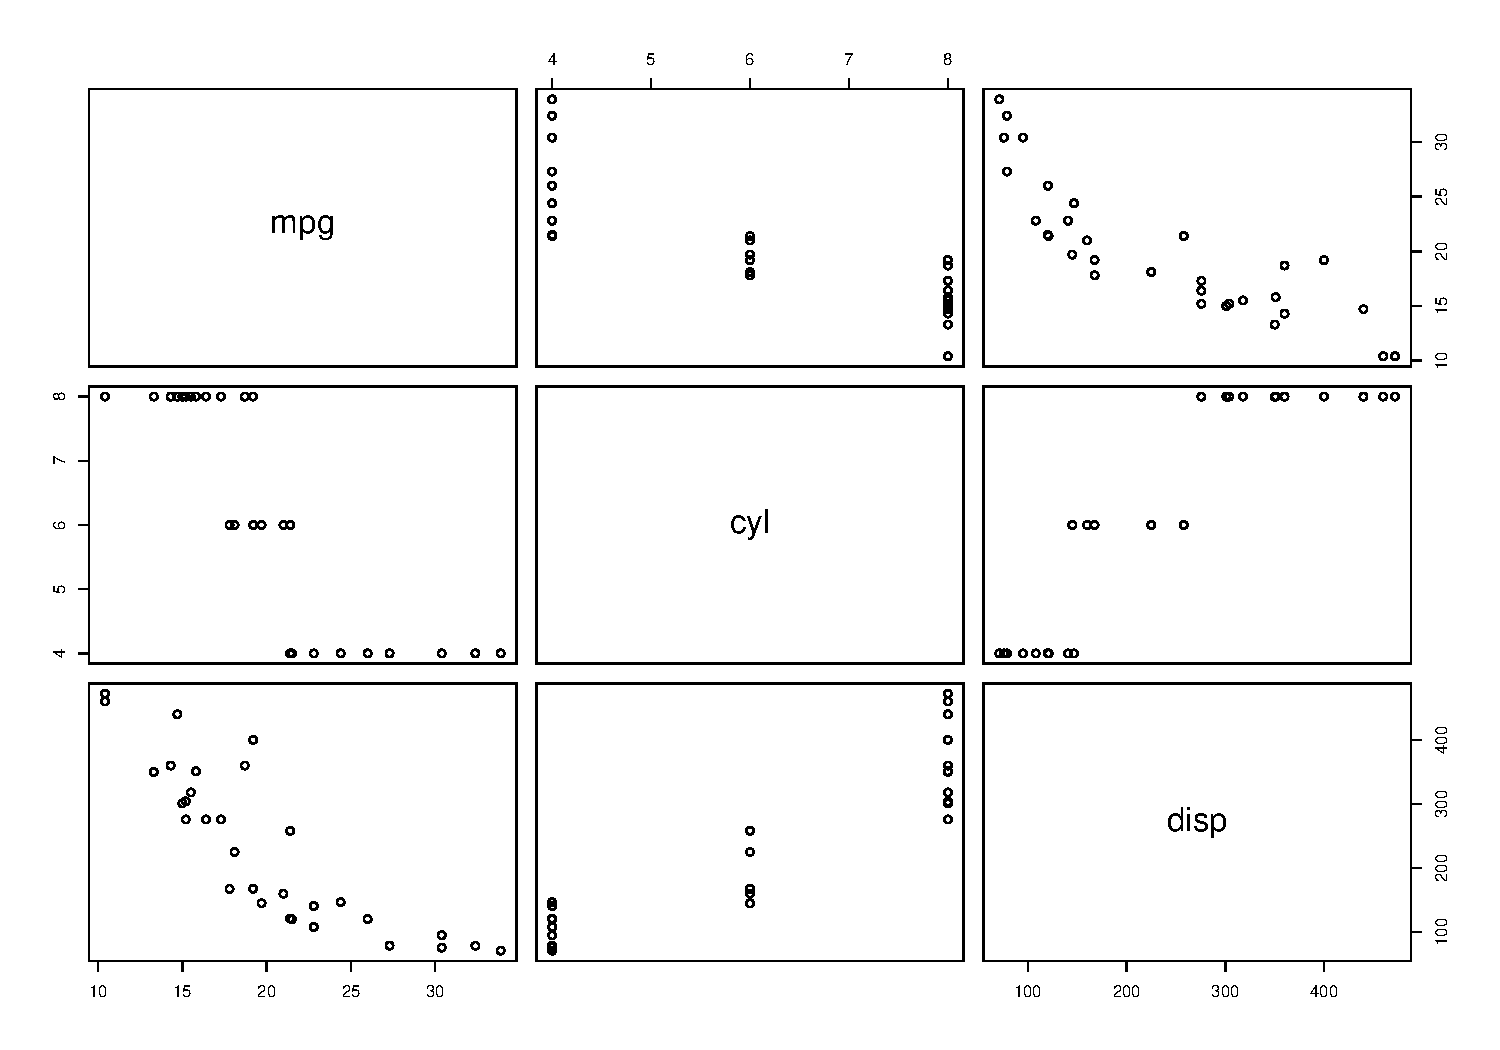
\includegraphics[width=1\linewidth]{crashcourse_slides_files/figure-beamer/unnamed-chunk-4-1}

\normalsize

\columnsend
\end{frame}

\begin{frame}[fragile]{Kan man gøre det hele \emph{endnu} nemmere?}
\protect\hypertarget{kan-man-guxf8re-det-hele-endnu-nemmere}{}
\begin{itemize}
\item
  Der er lavet et par \texttt{R}-pakker, der spytter ready-made kort ud
  for dig
\item
  \href{https://github.com/sebastianbarfort/mapDK}{\{mapDK\}} er
  efterhånden fem år gammel og er ikke rigtigt blevet opdateret. Den er
  et no-go
\item
  \href{https://github.com/kristianSN/plotDK}{\{plotDK\}} blev lanceret
  i 2021. Den kan meget af det samme, men er udgivet på \texttt{CRAN} og
  er up to date.
\item
  Min anke med de pakker er primært, at

  \begin{itemize}
  \item
    De (meget!) hurtigt bliver spændetrøjer ift. hvad man kan
    visualisere og hvordan
  \item
    Det faktisk er rigtig nemt at gøre det selv!
  \end{itemize}
\item
  Det er så det, vi er her for at snakke lidt om i dag!
\end{itemize}
\end{frame}

\hypertarget{the-basics-geodata-i-r}{%
\section{\texorpdfstring{The Basics: Geodata i
\texttt{R}}{The Basics: Geodata i R}}\label{the-basics-geodata-i-r}}

\begin{frame}[fragile]{A Blast from the past: \{\texttt{sp}\}}
\protect\hypertarget{a-blast-from-the-past-sp}{}
\tiny

\normalsize

\begin{itemize}
\item
  Det har tidligere været relativt besværligt at arbejde med spatialt
  data i \texttt{R}
\item
  \texttt{sp}-pakken var det førende framework, men selv simple datasæt
  var\ldots{} irriterende:
\end{itemize}

\begin{figure}[H]
    \centering
    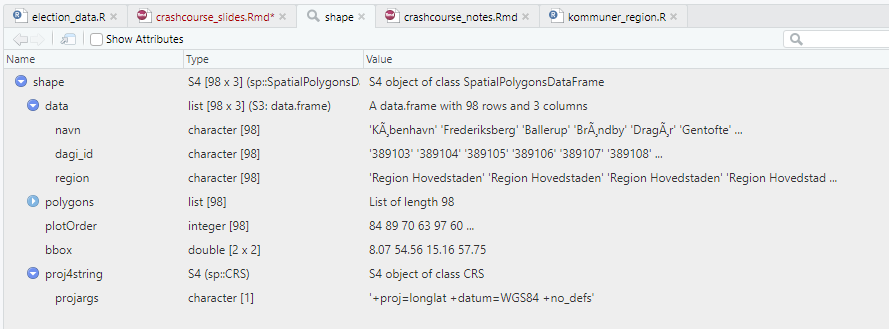
\includegraphics[width=.90\textwidth]{pictures/sp.png}
\end{figure}
\end{frame}

\begin{frame}[fragile]{Din nye bedste ven: \{\texttt{sf}\}}
\protect\hypertarget{din-nye-bedste-ven-sf}{}
\begin{itemize}
\item
  Med \texttt{sf} er det blevet
  \href{https://www.nickbearman.me.uk/2019/04/spatial-r-moving-from-sp-to-sf/}{smooth
  sailing}. Den måde, pakken håndterer det \emph{spatiale} aspekt af et
  datasæt gør, at det ligner alle andre datasæt til forveksling:
\item
  Magien ligger i \texttt{geometry}-listen til sidst. Alt (!) andet er
  data frames/tibbles, som I kender dem
\end{itemize}

\tiny

\begin{Shaded}
\begin{Highlighting}[]
\FunctionTok{library}\NormalTok{(tidyverse)}
\FunctionTok{library}\NormalTok{(sf)}

\NormalTok{df }\OtherTok{\textless{}{-}} \FunctionTok{st\_read}\NormalTok{(}\AttributeTok{dsn =} \StringTok{"data/kommuner"}\NormalTok{,}
              \AttributeTok{layer =} \StringTok{"kommuner"}\NormalTok{)}
\end{Highlighting}
\end{Shaded}

\normalsize

\tiny

\begin{Shaded}
\begin{Highlighting}[]
\NormalTok{df}
\end{Highlighting}
\end{Shaded}

\begin{verbatim}
## Simple feature collection with 98 features and 3 fields
## Geometry type: MULTIPOLYGON
## Dimension:     XY
## Bounding box:  xmin: 8.07251 ymin: 54.55908 xmax: 15.15738 ymax: 57.75257
## Geodetic CRS:  WGS 84
## First 10 features:
##             navn dagi_id             region                       geometry
## 1      København  389103 Region Hovedstaden MULTIPOLYGON (((12.54502 55...
## 2  Frederiksberg  389104 Region Hovedstaden MULTIPOLYGON (((12.53735 55...
## 3       Ballerup  389105 Region Hovedstaden MULTIPOLYGON (((12.3423 55....
## 4        Brøndby  389106 Region Hovedstaden MULTIPOLYGON (((12.44279 55...
## 5         Dragør  389107 Region Hovedstaden MULTIPOLYGON (((12.64513 55...
## 6       Gentofte  389108 Region Hovedstaden MULTIPOLYGON (((12.59175 55...
## 7       Gladsaxe  389109 Region Hovedstaden MULTIPOLYGON (((12.47771 55...
## 8       Glostrup  389110 Region Hovedstaden MULTIPOLYGON (((12.41842 55...
## 9         Herlev  389111 Region Hovedstaden MULTIPOLYGON (((12.40838 55...
## 10   Albertslund  389112 Region Hovedstaden MULTIPOLYGON (((12.36431 55...
\end{verbatim}

\normalsize
\end{frame}

\begin{frame}[fragile]{Din nye bedste ven: \{\texttt{sf}\}}
\protect\hypertarget{din-nye-bedste-ven-sf-1}{}
Helt konkret giver \texttt{sf} os mulighed for at bruge simple
\texttt{tidyverse}-funktioner til at:

\begin{enumerate}
\item
  arbejde med data (\texttt{dplyr}, \texttt{tidyr} osv.)
\item
  visualisere data! (\texttt{ggplot2})
\end{enumerate}

Lad os prøve begge dele!

\columnsbegin
\column{.5\textwidth}

\tiny

\begin{Shaded}
\begin{Highlighting}[]
\CommentTok{\# data wrangling med tidyverse (dplyr):}
\NormalTok{df }\OtherTok{\textless{}{-}}\NormalTok{ df }\SpecialCharTok{\%\textgreater{}\%} 
  \FunctionTok{filter}\NormalTok{(region }\SpecialCharTok{\%in\%} \FunctionTok{c}\NormalTok{(}\StringTok{"Region Syddanmark"}\NormalTok{, }\StringTok{"Region Midtjylland"}\NormalTok{))}

\CommentTok{\# data viz med tidyverse (ggplot2):}
\FunctionTok{ggplot}\NormalTok{() }\SpecialCharTok{+}
  \FunctionTok{geom\_sf}\NormalTok{(}\AttributeTok{data =}\NormalTok{ df, }\FunctionTok{aes}\NormalTok{(}\AttributeTok{fill =}\NormalTok{ region)) }\SpecialCharTok{+}
  \FunctionTok{theme\_void}\NormalTok{()}
\end{Highlighting}
\end{Shaded}

\normalsize

\column{.5\textwidth}

\tiny

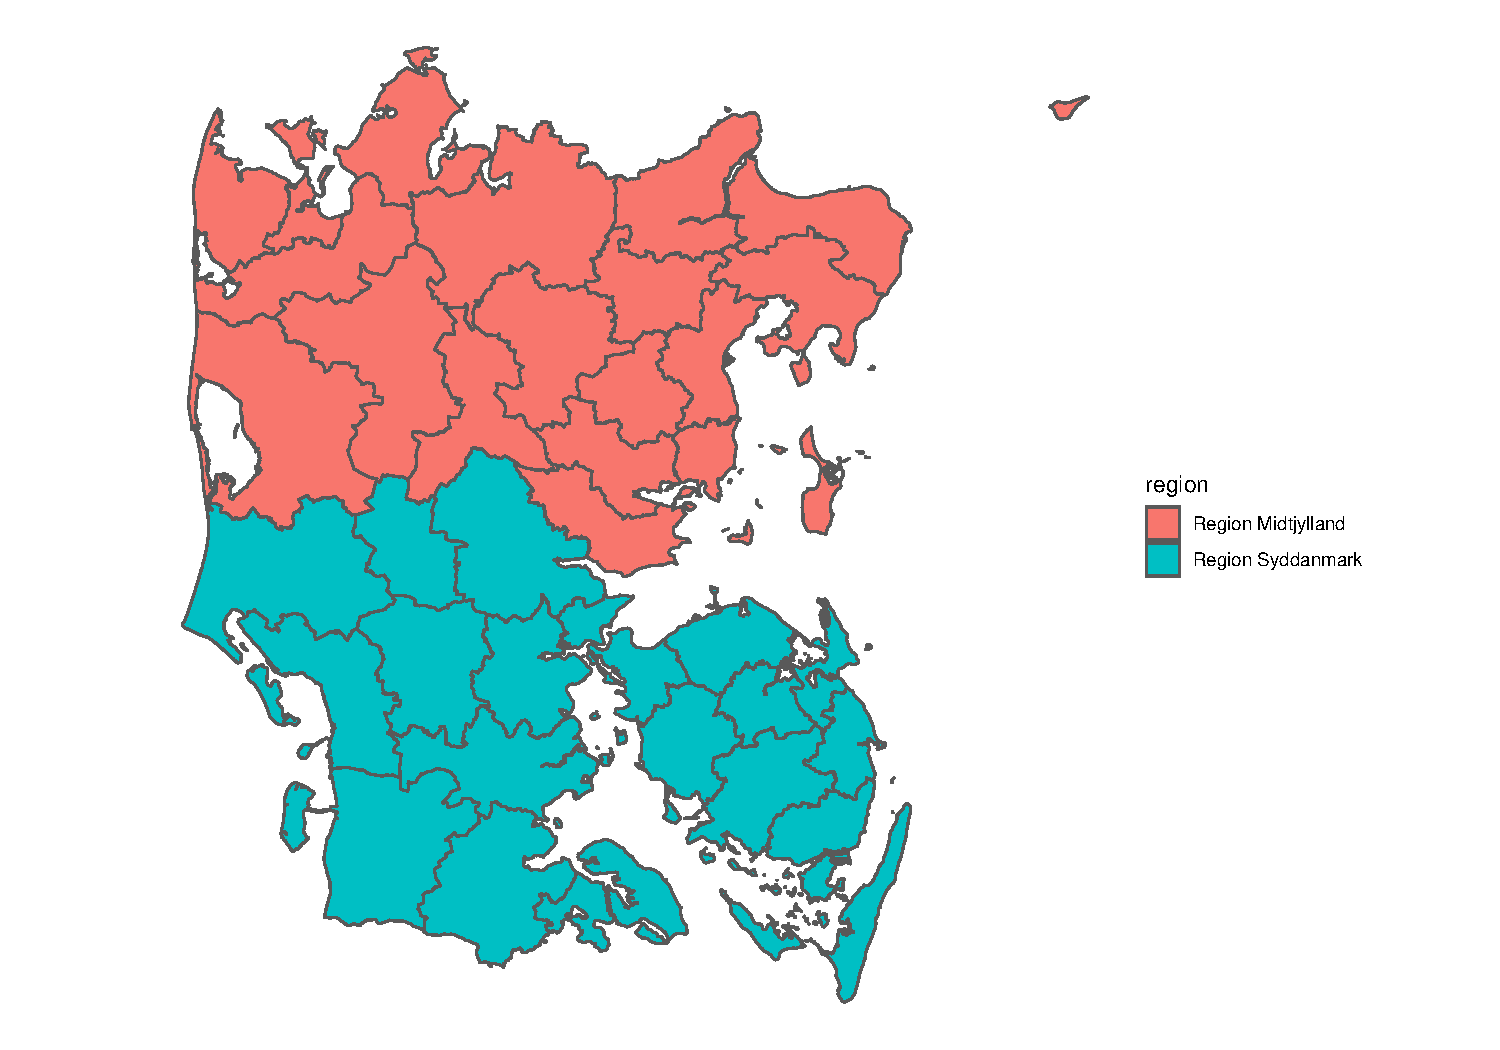
\includegraphics{crashcourse_slides_files/figure-beamer/unnamed-chunk-9-1.pdf}

\normalsize \columnsend
\end{frame}

\begin{frame}{Datastrukturer og typer af geodata}
\protect\hypertarget{datastrukturer-og-typer-af-geodata}{}
Grundlæggende arbejder vi med \textbf{tre typer af geospatiale
datakilder}

Hver type har en (nogenlunde) parallel til graftyper, I er vant til at
arbejde med:

\bigskip

\begin{enumerate}
\tightlist
\item
  \textbf{Punkter}
\end{enumerate}

\begin{itemize}
\tightlist
\item
  Tænk på dem som almindelige \emph{punkter i et scatterplot}
\end{itemize}

\begin{enumerate}
\setcounter{enumi}{1}
\tightlist
\item
  \textbf{Linjer}
\end{enumerate}

\begin{itemize}
\tightlist
\item
  Tænk på dem som \emph{linjer i et linechart}
\end{itemize}

\begin{enumerate}
\setcounter{enumi}{2}
\tightlist
\item
  \textbf{Polygoner}
\end{enumerate}

\begin{itemize}
\tightlist
\item
  Her er parallelen ikke lige så tydelig
\item
  \ldots{} men i en data viz-kontekst kan I tænke på dem som
  \emph{søjler i et bar chart} (ish\ldots)
\end{itemize}
\end{frame}

\begin{frame}{(1) Punkter}
\protect\hypertarget{punkter}{}
\columnsbegin
\column{.4\textwidth}

\begin{itemize}
\item
  Punkter består af simple koordinater (x, y), der refererer til en
  specifik lokation
\item
  Punkter har ingen størrelse (og intet \emph{areal}), de er uendeligt
  små
\item
  Eksempler: byer, stationer, skoler osv.
\end{itemize}

\column{.6\textwidth}

\tiny

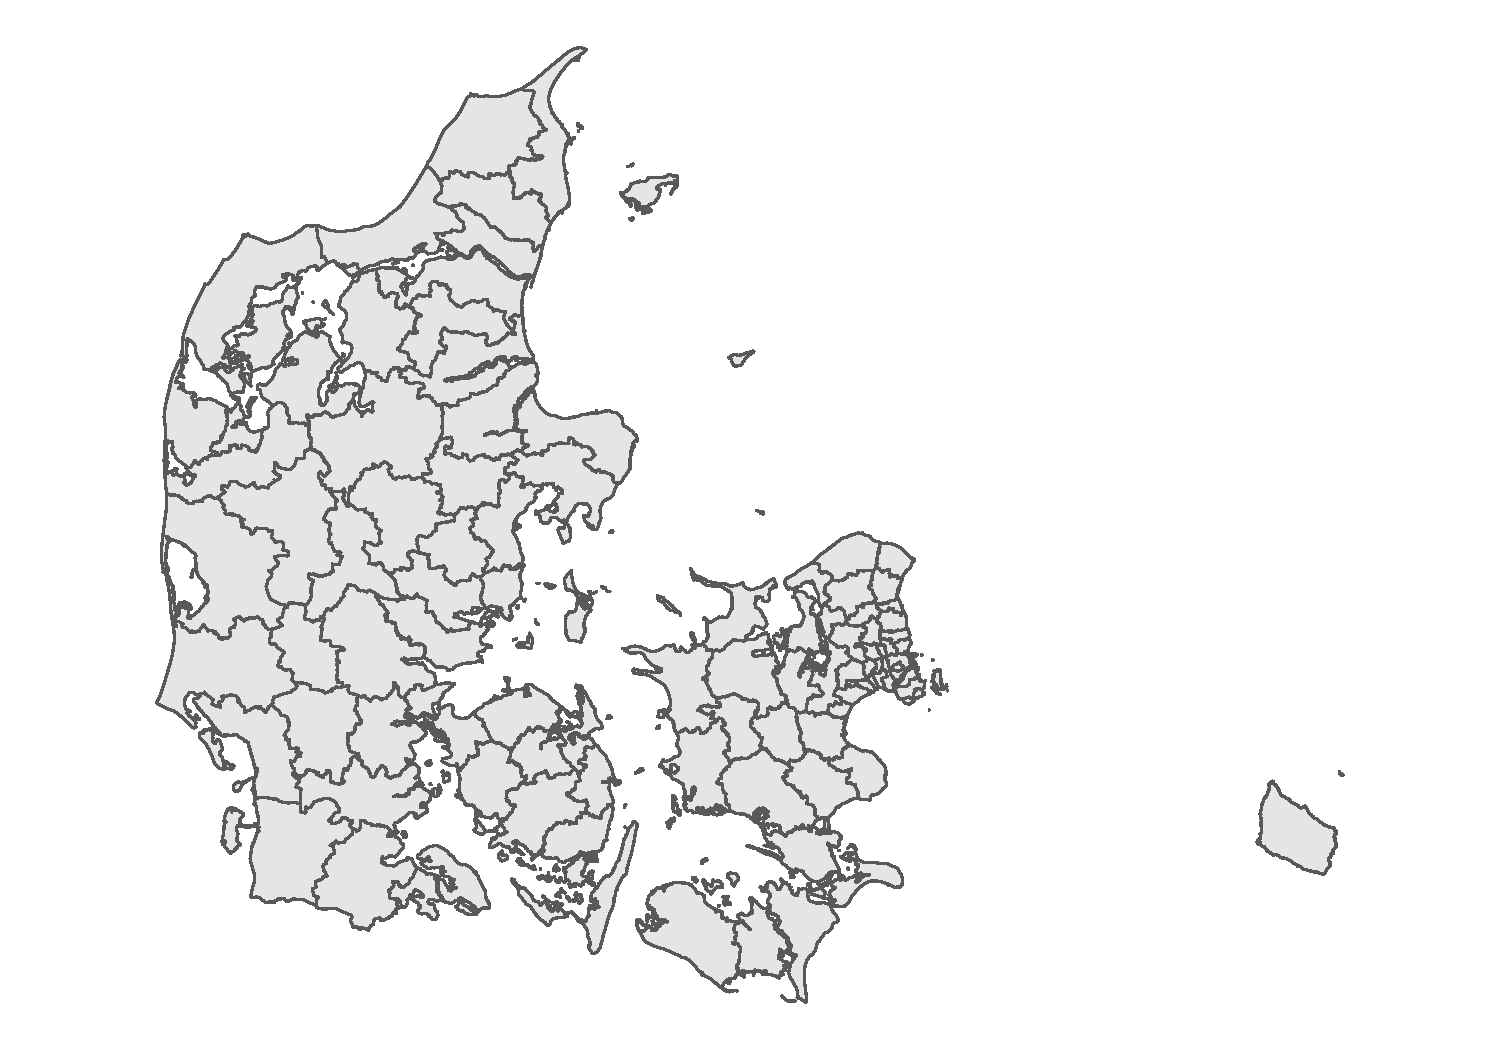
\includegraphics[width=1\linewidth]{crashcourse_slides_files/figure-beamer/unnamed-chunk-10-1}

\normalsize

\columnsend
\end{frame}

\begin{frame}{(2) Linjer}
\protect\hypertarget{linjer}{}
\columnsbegin
\column{.4\textwidth}

\begin{itemize}
\item
  Linjer består -- grundlæggende -- af punkter, der er kombineret til en
  \emph{linestring} vha. en defineret rækkefølge
\item
  Konstruktionen er sjældent noget, I skal bekymre jer om: linjedata
  ligger typisk opbevaret som linjer (\(\neq\) punkter). Her er det bare
  plug 'n play
\item
  Linjer har intet \emph{areal} (fordi de består af punkter)
\item
  Eksempler: veje, floder, jernbanenetværk osv.
\end{itemize}

\column{.6\textwidth}

\tiny

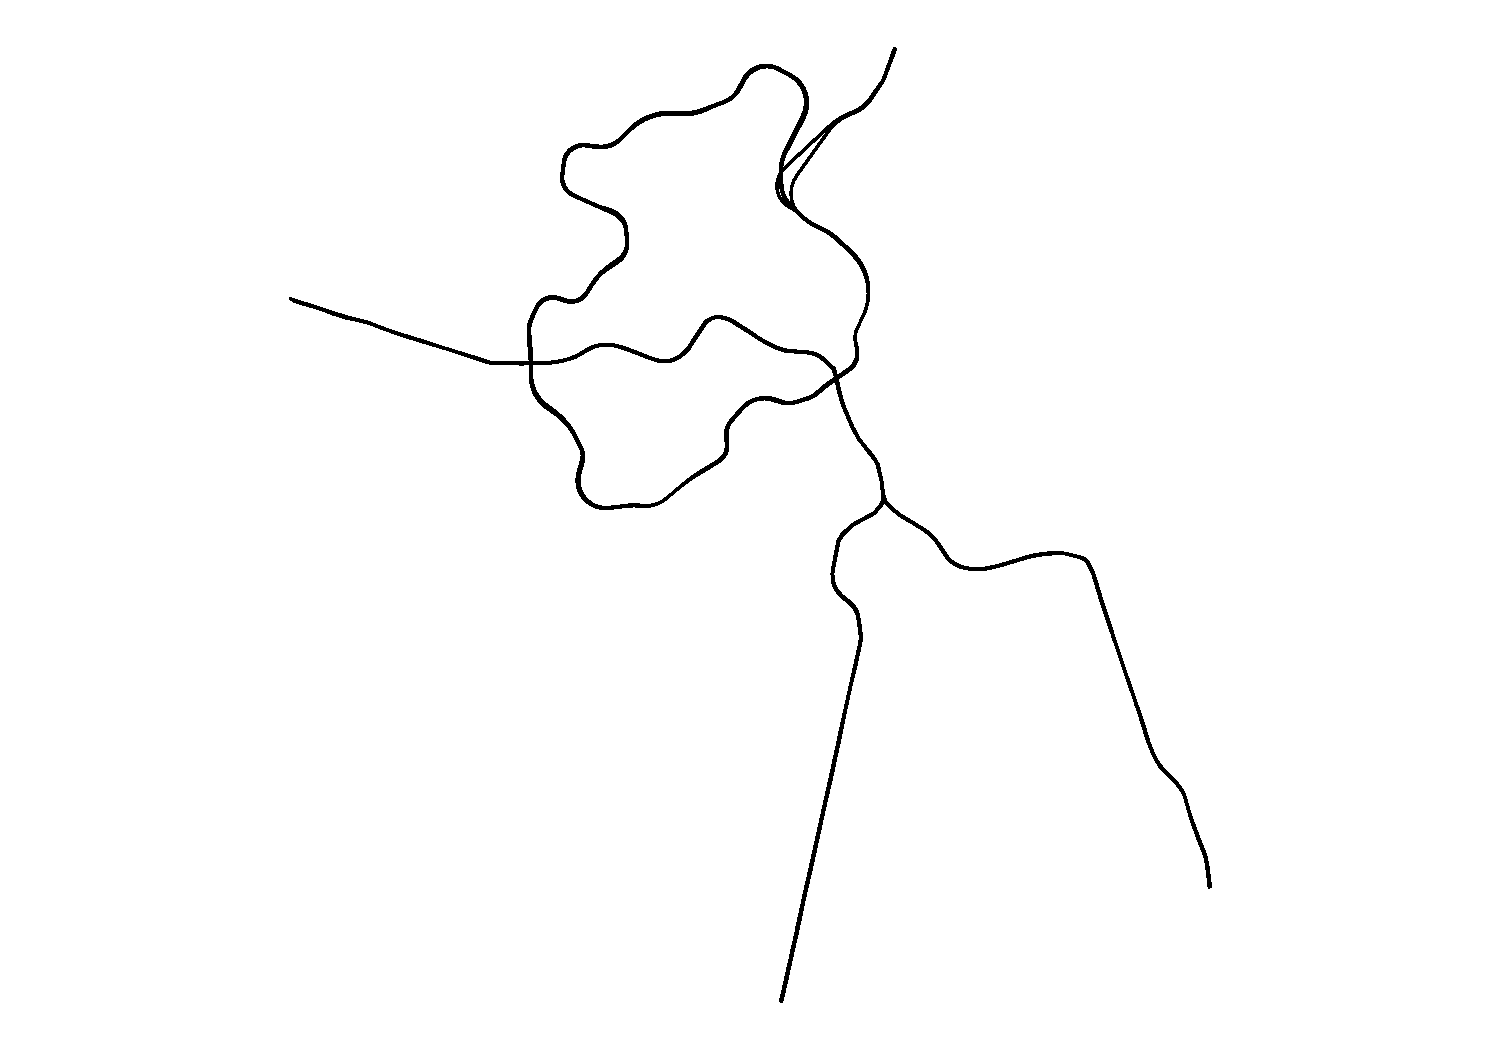
\includegraphics[width=1\linewidth]{crashcourse_slides_files/figure-beamer/unnamed-chunk-11-1}

\normalsize

\columnsend
\end{frame}

\begin{frame}{(3) Polygoner}
\protect\hypertarget{polygoner}{}
\columnsbegin
\column{.4\textwidth}

\begin{itemize}
\item
  Polygoner består -- ligesom linjer -- af punkter, der er kombineret
  til en \emph{polygon} vha. en defineret rækkefølge. Igen, det er
  sjældent noget, I skal bekymre jer om
\item
  Forskellen er, at polygoner er \emph{lukkede linjer}, der former et
  afgrænset område
\item
  De kan have alle tænkelige former. Det centrale er, at polygoner har
  et \emph{areal}
\item
  Eksempler: stater, kommuner, valgkredse osv.
\end{itemize}

\column{.6\textwidth}

\tiny

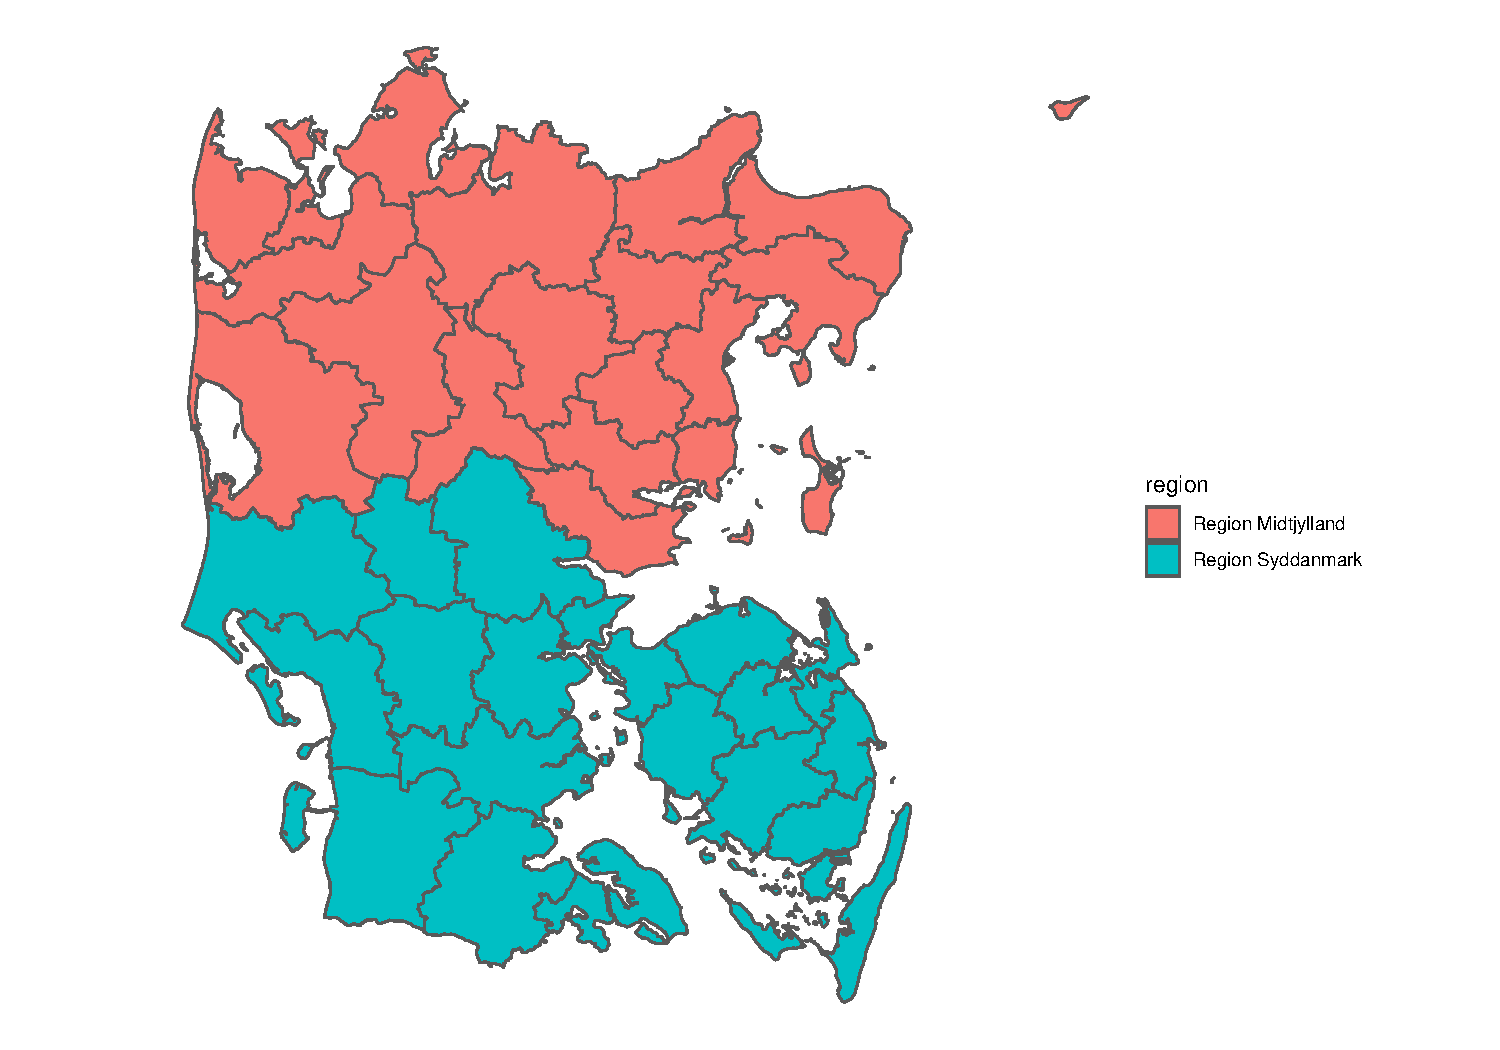
\includegraphics[width=1\linewidth]{crashcourse_slides_files/figure-beamer/unnamed-chunk-12-1}

\normalsize

\columnsend
\end{frame}

\hypertarget{geospatial-datavisualisering}{%
\section{Geospatial
datavisualisering}\label{geospatial-datavisualisering}}

\begin{frame}[fragile]{Visualisering med \{\texttt{ggplot2}\}}
\protect\hypertarget{visualisering-med-ggplot2}{}
XXX

\tiny

\begin{Shaded}
\begin{Highlighting}[]
\NormalTok{vshare }\OtherTok{\textless{}{-}} \FunctionTok{st\_read}\NormalTok{(}\AttributeTok{dsn =} \StringTok{"data/kommuner\_98"}\NormalTok{,}
                  \AttributeTok{layer =} \StringTok{"kommuner\_98"}\NormalTok{)}
\end{Highlighting}
\end{Shaded}

\normalsize

\tiny

\begin{Shaded}
\begin{Highlighting}[]
\FunctionTok{class}\NormalTok{(vshare}\SpecialCharTok{$}\NormalTok{geometry)}
\end{Highlighting}
\end{Shaded}

\begin{verbatim}
## [1] "sfc_MULTIPOLYGON" "sfc"
\end{verbatim}

\normalsize

YYY

\tiny

\begin{Shaded}
\begin{Highlighting}[]
\NormalTok{barns }\OtherTok{\textless{}{-}} \FunctionTok{st\_read}\NormalTok{(}\AttributeTok{dsn =} \StringTok{"data/barns"}\NormalTok{,}
                 \AttributeTok{layer =} \StringTok{"barns"}\NormalTok{)}
\end{Highlighting}
\end{Shaded}

\normalsize

\tiny

\begin{Shaded}
\begin{Highlighting}[]
\FunctionTok{class}\NormalTok{(barns}\SpecialCharTok{$}\NormalTok{geometry)}
\end{Highlighting}
\end{Shaded}

\begin{verbatim}
## [1] "sfc_POINT" "sfc"
\end{verbatim}

\normalsize
\end{frame}

\begin{frame}[fragile]{Visualisering med \{\texttt{ggplot2}\}}
\protect\hypertarget{visualisering-med-ggplot2-1}{}
\onslide <1>
\columnsbegin
\column{.5\textwidth}

\tiny

\begin{Shaded}
\begin{Highlighting}[]
\FunctionTok{ggplot}\NormalTok{() }\SpecialCharTok{+}
  \FunctionTok{geom\_sf}\NormalTok{(}\AttributeTok{data =}\NormalTok{ vshare)}
\end{Highlighting}
\end{Shaded}

\normalsize \column{.5\textwidth}

\tiny

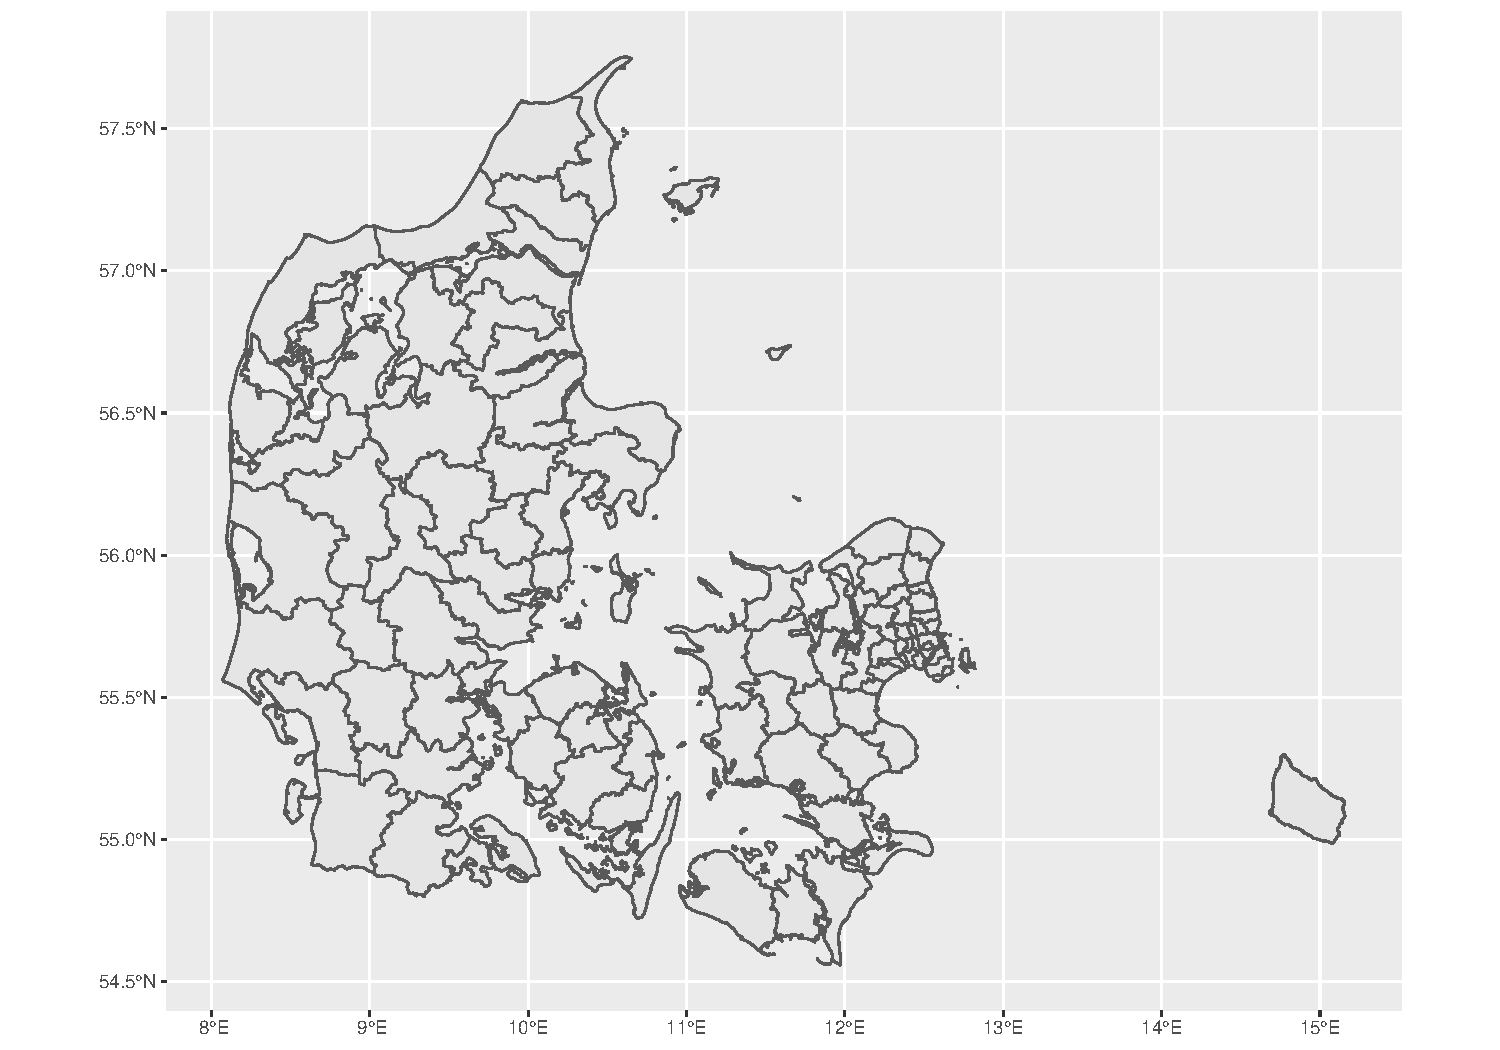
\includegraphics{crashcourse_slides_files/figure-beamer/unnamed-chunk-18-1.pdf}

\normalsize \columnsend

\onslide <2>
\columnsbegin
\column{.5\textwidth}

\tiny

\begin{Shaded}
\begin{Highlighting}[]
\FunctionTok{ggplot}\NormalTok{() }\SpecialCharTok{+}
  \FunctionTok{geom\_sf}\NormalTok{(}\AttributeTok{data =}\NormalTok{ vshare) }\SpecialCharTok{+}
  \FunctionTok{theme\_void}\NormalTok{()}
\end{Highlighting}
\end{Shaded}

\normalsize \column{.5\textwidth}

\tiny

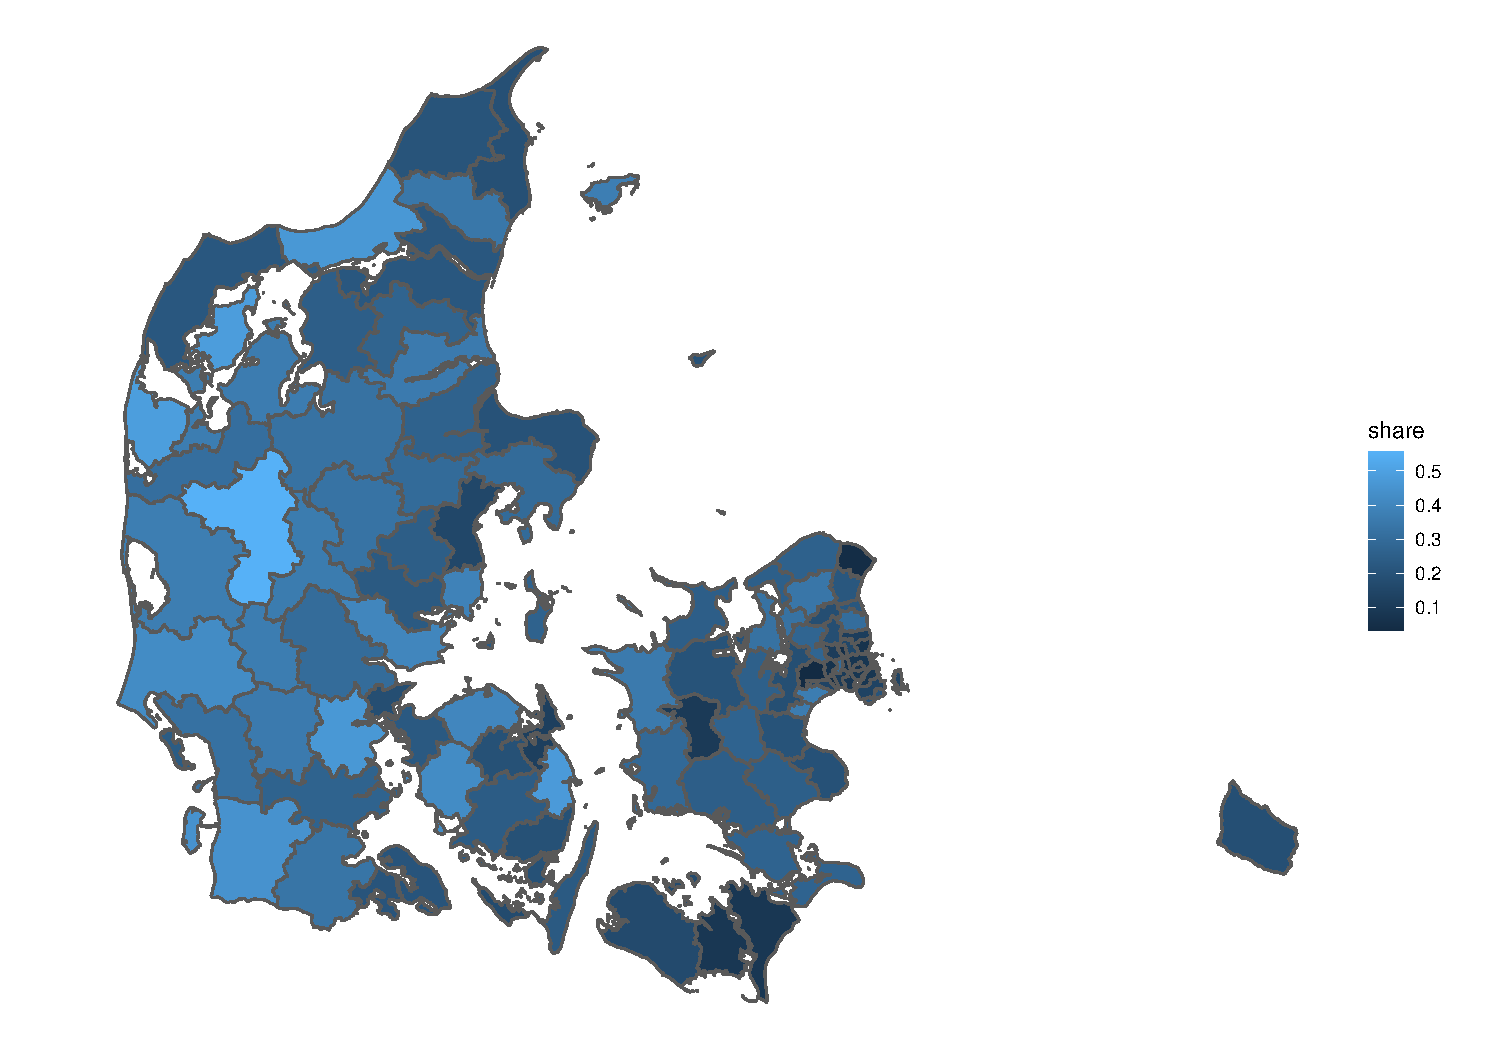
\includegraphics{crashcourse_slides_files/figure-beamer/unnamed-chunk-20-1.pdf}

\normalsize \columnsend
\end{frame}

\hypertarget{datakilder}{%
\section{Datakilder}\label{datakilder}}

\begin{frame}{DAGI}
\protect\hypertarget{dagi}{}
\columnsbegin

\column{.6\textwidth}

\begin{itemize}
\tightlist
\item
  \emph{``\textbf{Danmarks Administrative Geografiske Inddeling (DAGI)}
  beskriver landets administrative og geografiske inddeling i kommuner,
  regioner, sogne, retskredse, politikredse, postnumre,
  opstillingskredse og lignende.''} --
  \href{https://dawadocs.dataforsyningen.dk/dok/dagi}{DAWA}
\end{itemize}

\medskip

\begin{itemize}
\item
  \ldots{} med andre ord; alt hvad vi kunne drømme om
\item
  DAGI-data kan hentes via Styrelsen for Dataforsyning og
  Effektiviserings
  \href{https://datafordeler.dk/dataoversigt/}{Datafordeler}
\item
  Det er en ret håbløs hjemmeside, til gengæld er der masser at vælge
  mellem (inkl. historiske enheder!)
\end{itemize}

\column{.4\textwidth}

\begin{figure}[H]
    \centering
    
\includegraphics[width=.90\textwidth]{pictures/logo_sdfe.png}
\end{figure}

\columnsend
\end{frame}

\begin{frame}{DAGI}
\protect\hypertarget{dagi-1}{}
\begin{itemize}
\item
  Til de fleste formål kan vi hoppe uden om Datafordelen ved at bruge
  \href{https://dawadocs.dataforsyningen.dk/dok/dagi}{DAWA (Danmarks
  Adressers Web API)} og den
  \href{https://dawadocs.dataforsyningen.dk/dok/api\#dagi}{tilhørende
  API}
\item
  API'en er plug 'n play, hvor vi kan vælge de
  \textcolor{purple}{enheder}, vi skal bruge, og specificere
  \textcolor{teal}{format}:
\item
  \nolinkurl{https://api.dataforsyningen.dk/ \textcolor{purple}{kommuner}?format=\textcolor{teal}{geojson}}
\end{itemize}
\end{frame}

\begin{frame}[fragile]{DAGI: et eksempel}
\protect\hypertarget{dagi-et-eksempel}{}
\columnsbegin
\column{.5\textwidth}

\tiny

\begin{Shaded}
\begin{Highlighting}[]
\CommentTok{\# definér data}
\NormalTok{url }\OtherTok{\textless{}{-}} 
  \StringTok{"https://api.dataforsyningen.dk/kommuner?format=geojson"}

\CommentTok{\# indlæs data}
\NormalTok{kommuner\_raw }\OtherTok{\textless{}{-}} 
  \FunctionTok{read\_sf}\NormalTok{(url)}

\CommentTok{\# plot data}
\FunctionTok{ggplot}\NormalTok{() }\SpecialCharTok{+}
  \FunctionTok{geom\_sf}\NormalTok{(}\AttributeTok{data =}\NormalTok{ kommuner\_raw) }\SpecialCharTok{+}
  \FunctionTok{theme\_void}\NormalTok{()}
\end{Highlighting}
\end{Shaded}

\normalsize \column{.5\textwidth}

\tiny

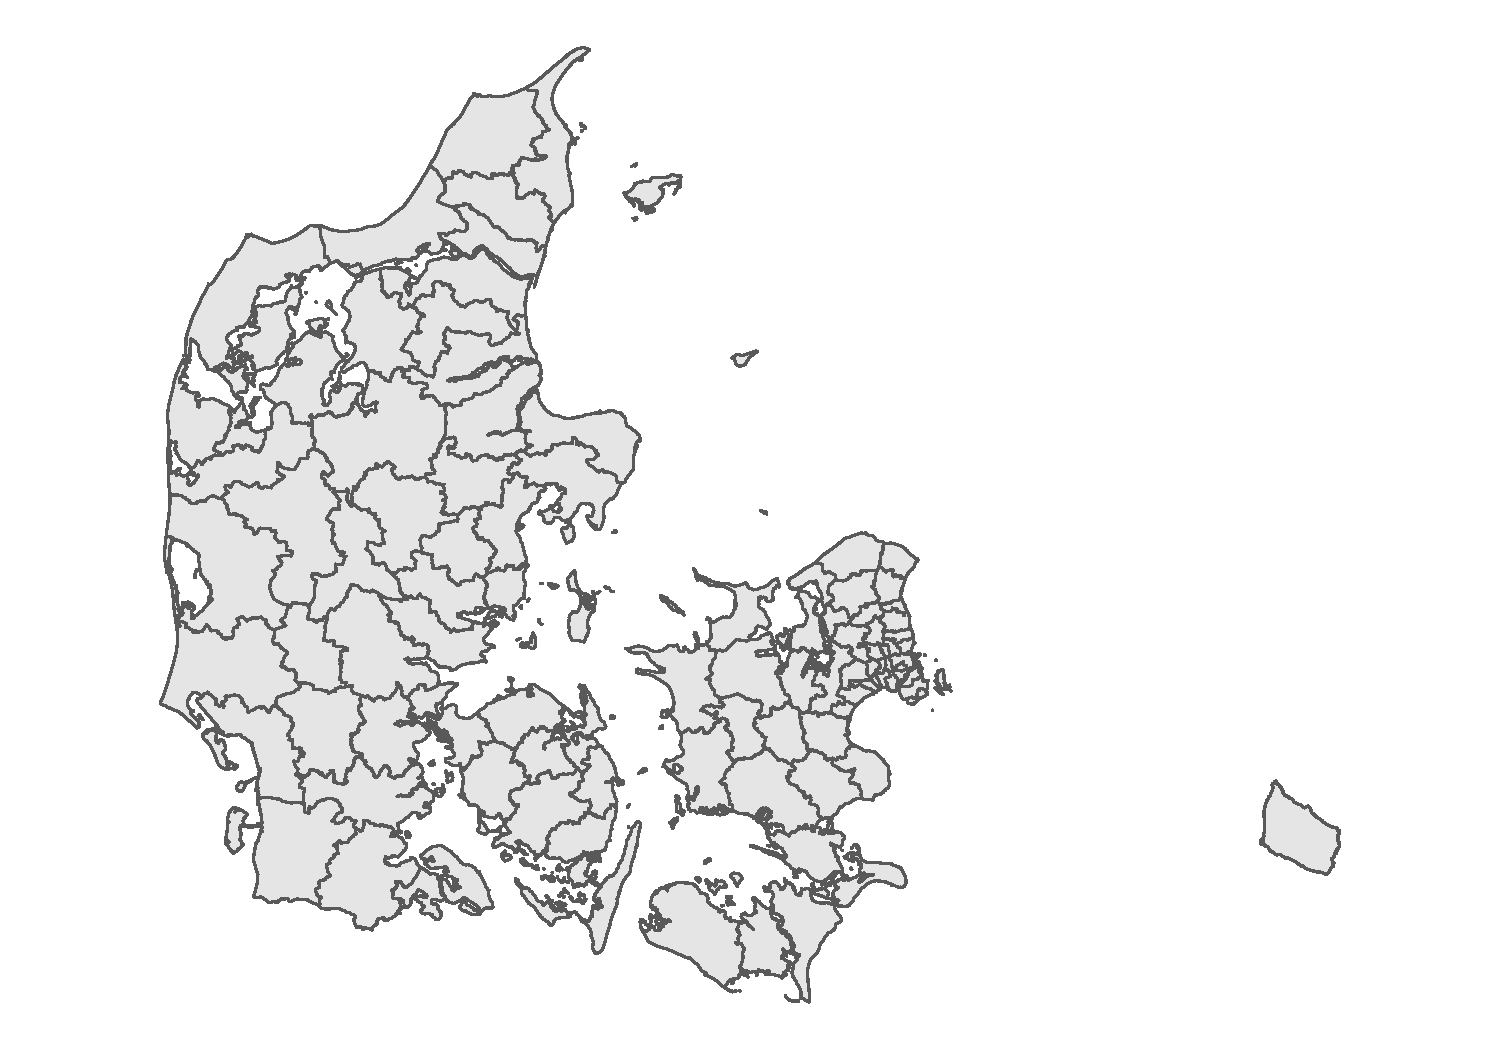
\includegraphics{crashcourse_slides_files/figure-beamer/unnamed-chunk-22-1.pdf}

\normalsize \columnsend
\end{frame}

\begin{frame}{OpenStreetMap}
\protect\hypertarget{openstreetmap}{}
\columnsbegin

\column{.6\textwidth}

\begin{itemize}
\item
  \href{https://www.openstreetmap.org/about}{OpenStreetMap (OSM)} er en
  crowd sourced geografisk database med detaljeret information om hele
  verden
\item
  OSM indeholder data på (næsten) alt, hvad hjertet begærer
\item
  OSM har en tilhørende
  \href{https://wiki.openstreetmap.org/wiki/Map_features}{wiki}, med en
  oversigt over de forskellige features
\end{itemize}

\column{.4\textwidth}

\begin{figure}[H]
    \centering
    
\includegraphics[width=.75\textwidth]{pictures/Openstreetmap_logo.svg}
\end{figure}

\columnsend
\end{frame}

\begin{frame}[fragile]{OpenStreetMap}
\protect\hypertarget{openstreetmap-1}{}
\columnsbegin

\column{.6\textwidth}

\begin{itemize}
\item
  Vi kan bruge R-pakken
  \href{https://cran.r-project.org/web/packages/osmdata/vignettes/osmdata.html}{\{\texttt{osmdata}\}}
  til at hente OSM-data direkte i \texttt{R}
\item
  Her skal vi bruge

  \begin{itemize}
  \tightlist
  \item
    En geografisk afgrænsning
  \item
    Valg af features (vha. argumenterne \texttt{key} og \texttt{value}):
  \end{itemize}
\end{itemize}

\column{.4\textwidth}

\begin{figure}[H]
    \centering
    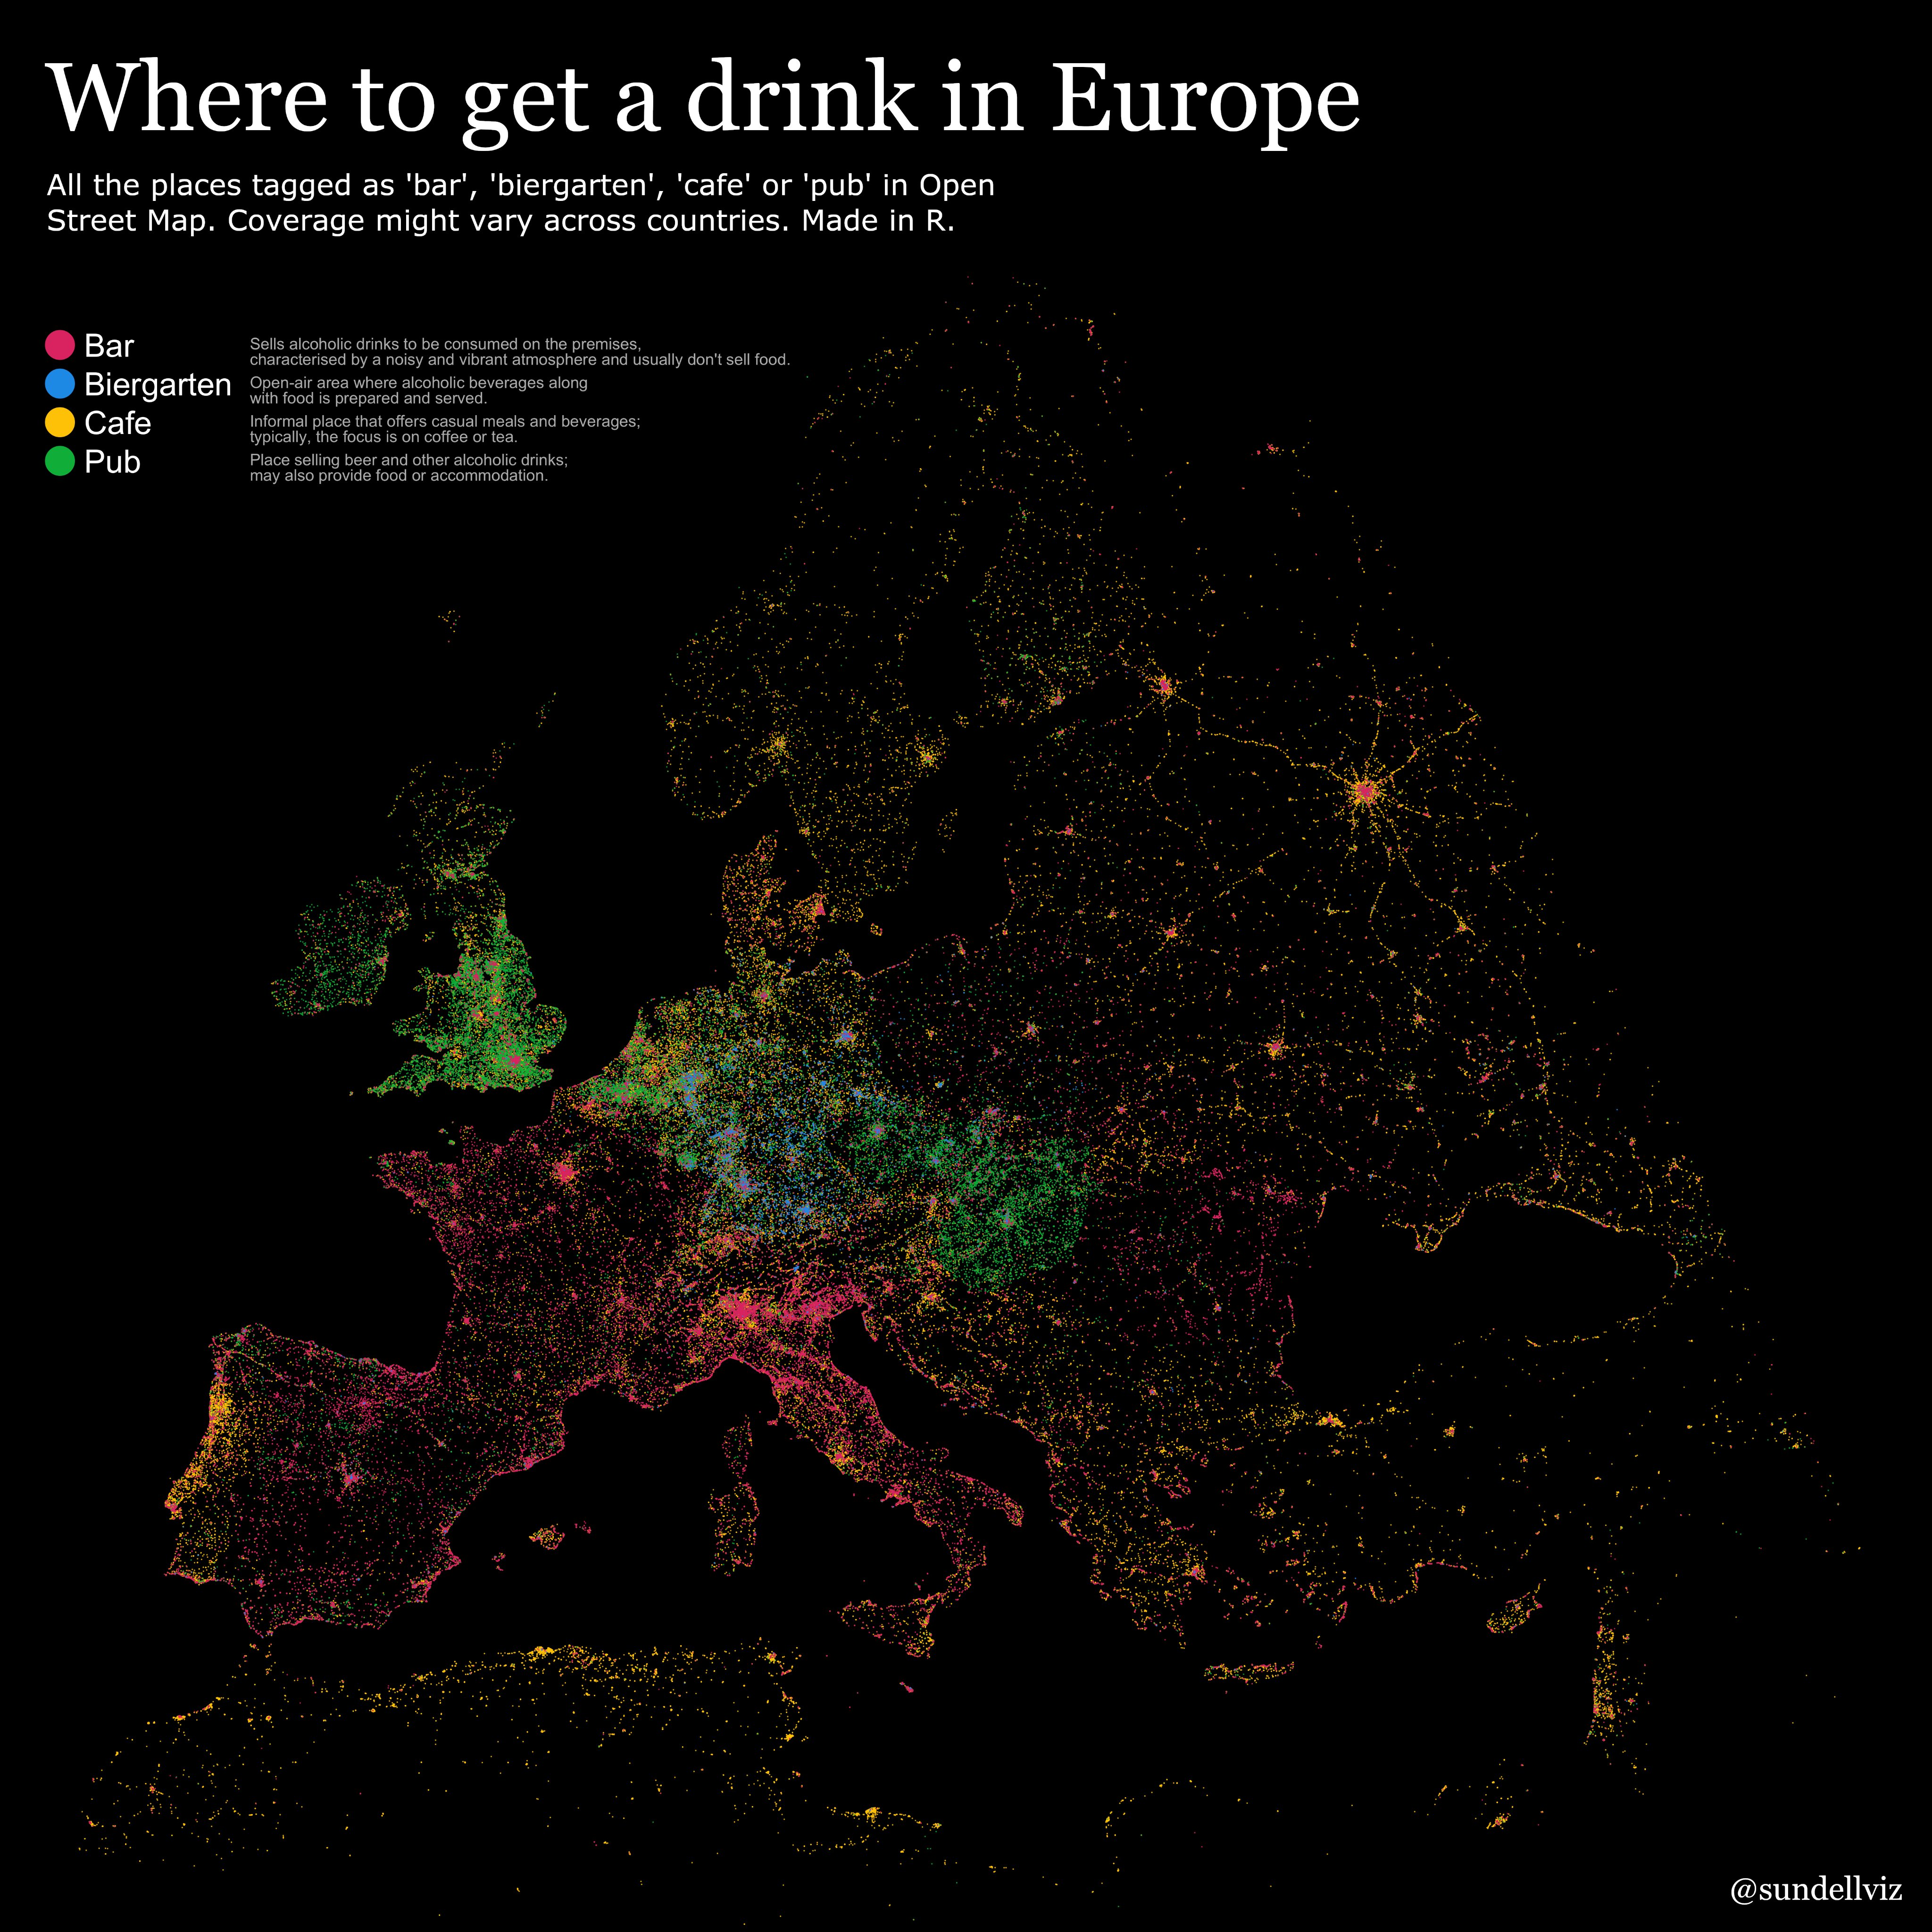
\includegraphics[width=.90\textwidth]{pictures/sundell_bars.png}
\end{figure}

\columnsend
\end{frame}

\begin{frame}[fragile]{OpenStreetMap: et eksempel}
\protect\hypertarget{openstreetmap-et-eksempel}{}
\columnsbegin
\column{.5\textwidth}

\tiny

\begin{Shaded}
\begin{Highlighting}[]
\FunctionTok{library}\NormalTok{(osmdata)}

\CommentTok{\# Hent OSM{-}data for Vejle}
\NormalTok{vejle }\OtherTok{\textless{}{-}}\NormalTok{ kommuner\_raw }\SpecialCharTok{\%\textgreater{}\%} 
  \FunctionTok{filter}\NormalTok{(navn }\SpecialCharTok{==} \StringTok{"Vejle"}\NormalTok{)}

\NormalTok{vejle\_bbox }\OtherTok{\textless{}{-}}\NormalTok{ vejle }\SpecialCharTok{\%\textgreater{}\%} 
  \FunctionTok{st\_bbox}\NormalTok{()}

\NormalTok{osm }\OtherTok{\textless{}{-}}\NormalTok{ vejle\_bbox }\SpecialCharTok{\%\textgreater{}\%} 
  \FunctionTok{opq}\NormalTok{()}

\CommentTok{\# Hent udvalgte veje}
\NormalTok{roads }\OtherTok{\textless{}{-}}\NormalTok{ osm }\SpecialCharTok{\%\textgreater{}\%} 
  \FunctionTok{add\_osm\_feature}\NormalTok{(}\AttributeTok{key =} \StringTok{\textquotesingle{}highway\textquotesingle{}}\NormalTok{,}
                  \AttributeTok{value =} \FunctionTok{c}\NormalTok{(}\StringTok{\textquotesingle{}motorway\textquotesingle{}}\NormalTok{, }\StringTok{\textquotesingle{}trunk\textquotesingle{}}\NormalTok{,}
                            \StringTok{\textquotesingle{}primary\textquotesingle{}}\NormalTok{, }\StringTok{\textquotesingle{}secondary\textquotesingle{}}\NormalTok{, }
                            \StringTok{\textquotesingle{}tertiary\textquotesingle{}}\NormalTok{)) }\SpecialCharTok{\%\textgreater{}\%} 
  \FunctionTok{osmdata\_sf}\NormalTok{()}

\CommentTok{\# Beskær}
\NormalTok{roads }\OtherTok{\textless{}{-}}\NormalTok{ roads}\SpecialCharTok{$}\NormalTok{osm\_lines }\SpecialCharTok{\%\textgreater{}\%} 
  \FunctionTok{st\_intersection}\NormalTok{(., vejle)}

\CommentTok{\# Plot vejene}
\FunctionTok{ggplot}\NormalTok{() }\SpecialCharTok{+}
  \FunctionTok{geom\_sf}\NormalTok{(}\AttributeTok{data =}\NormalTok{ vejle, }\AttributeTok{fill =} \StringTok{"white"}\NormalTok{) }\SpecialCharTok{+}
  \FunctionTok{geom\_sf}\NormalTok{(}\AttributeTok{data =}\NormalTok{ roads, }\FunctionTok{aes}\NormalTok{(}\AttributeTok{color =} \FunctionTok{as.numeric}\NormalTok{(maxspeed))) }\SpecialCharTok{+}
  \FunctionTok{scale\_color\_viridis\_c}\NormalTok{(}\AttributeTok{direction =} \SpecialCharTok{{-}}\DecValTok{1}\NormalTok{, }\AttributeTok{name =} \StringTok{"Speed limit (km/h)"}\NormalTok{) }\SpecialCharTok{+}
  \FunctionTok{theme\_void}\NormalTok{()}
\end{Highlighting}
\end{Shaded}

\normalsize \column{.5\textwidth}

\tiny

\begin{verbatim}
## Data (c) OpenStreetMap contributors, ODbL 1.0. https://www.openstreetmap.org/copyright
\end{verbatim}

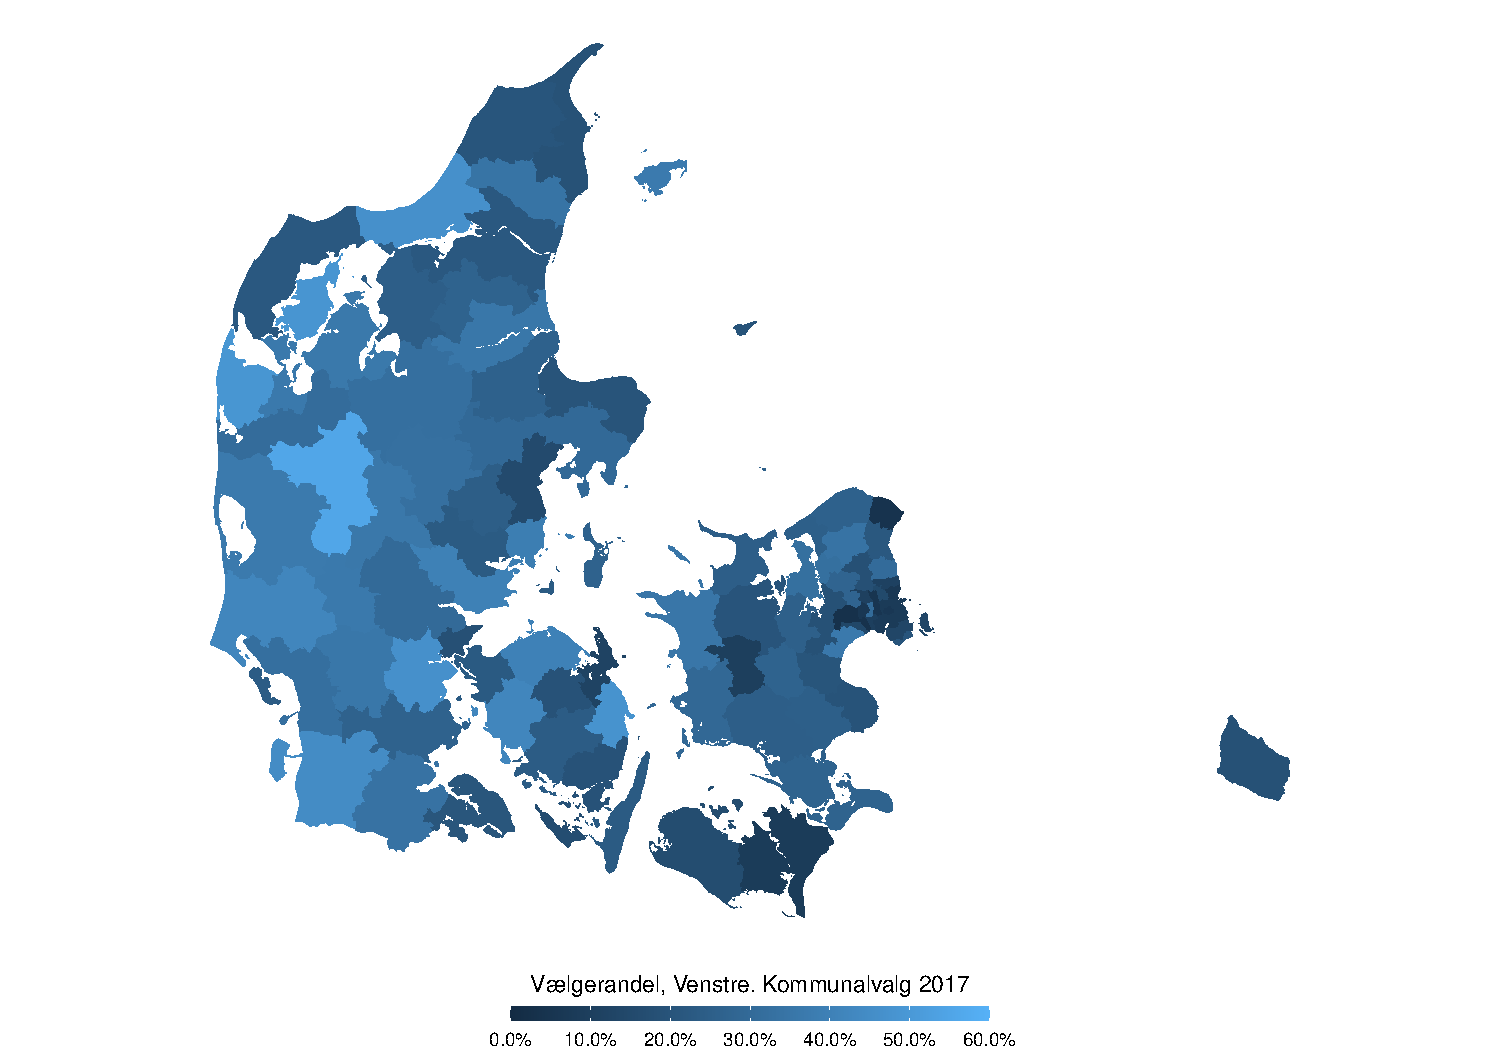
\includegraphics{crashcourse_slides_files/figure-beamer/unnamed-chunk-24-1.pdf}

\normalsize \columnsend
\end{frame}

\hypertarget{vuxe6rktuxf8jer-i-r}{%
\section{\texorpdfstring{Værktøjer i
\texttt{R}}{Værktøjer i R}}\label{vuxe6rktuxf8jer-i-r}}

\begin{frame}{text}
\protect\hypertarget{text}{}
xx
\end{frame}

\end{document}
